\chapter{Quasistationäre Felder}\label{quasistat}
Im vollen Satz der Maxwell-Gleichungen ($\nearrow$\ref{ind},\ref{quellf},\ref{durchf},\ref{gauss}) wurden Zeitableitungen bisher vernachlässigt. Nun soll der Fall betrachtet werden, dass \textbf{einer} der Terme $\textcolor{green}{\frac{\partial \vec{B} }{\partial t}}$ (Induktion) oder $\textcolor{red}{\frac{\partial \vec{D} }{\partial t}}$ (Verschiebungsstromdichte) vernachlässigt werden kann. Dies liefert \textbf{keine elektromagnetischen Wellen} ($\nearrow$ \ref{emwellen}) als Lösung! In der \textbf{Magneto-Quasistatik} wird der Verschiebungsstrom vernachlässigt, also 
\begin{equation}\label{annmqs}
	\textcolor{red}{\frac{\partial \vec{D} }{\partial t}} = \vec{0}\quad\text{ oder }\quad\left|\textcolor{red}{\frac{\partial \vec{D} }{\partial t}}\right|\ll |\vec{J}| \quad\text{ und }\quad \textcolor{green}{\frac{\partial \vec{B} }{\partial t}}\neq\vec{0}
\end{equation}
In der \textbf{Elektro-Quasistatik} wird die Induktion vernachlässigt, also 
\begin{equation}\label{anneqs}
\textcolor{green}{\frac{\partial \vec{B} }{\partial t}}=\vec{0} \quad \text{ und } \quad \textcolor{red}{\frac{\partial \vec{D} }{\partial t}} \neq \vec{0}
\end{equation}
 Quasistatische Probleme treten meist im Zusammenhang mit \textbf{technischen Quellen} auf.  Es ist daher naheliegend, alle Größen im \textbf{Frequenzbereich} darzustellen und beliebige Zeitabhängigkeiten im Sinne von \textbf{Fourier-Reihen/Fourier-Transformationen} darzustellen. \textbf{Komplexe Feldgrößen} ($i$-te Komponente der Fourier-Reihe):
		        \begin{equation}\label{frequenzbereich}\begin{split}
				        \vec{E}_i(\vec{r} ,\,t) &= \hat{\vec{E}}_i(\vec{r} )  \cos(\omega_i  t + \varphi_{E,i}) = \re{\hat{\vec{E}}_i(\vec{r} )  \mathrm{e}^{\mathrm{j} (\omega_i  t +  \varphi_{E,i})} } = \re{\ubar{\vec{E}}_i(\vec{r} )  \mathrm{e}^{\mathrm{j} \omega_i  t } }\\
				        \vec{H}_i(\vec{r} ,\,t) &= \hat{\vec{H}}_i(\vec{r} )  \cos(\omega_i  t + \varphi_{H,i}) = \re{\hat{\vec{H}}_i(\vec{r} )  \mathrm{e}^{\mathrm{j} (\omega_i  t +  \varphi_{H,i})} } = \re{\ubar{\vec{H}}_i(\vec{r} )  \mathrm{e}^{\mathrm{j} \omega_i  t } }
			        \end{split}\end{equation}
		  Dabei werden die \textbf{Phasoren} (ruhenden Zeiger) eingeführt:
		        \begin{equation}\label{phasoren}\begin{split}
				        \ubar{\vec{E}}_i(\vec{r} ) &= \hat{\vec{E}}_i(\vec{r} ) \cdot  \mathrm{e}^{\mathrm{j} \varphi_{E,i}} \\
				        \ubar{\vec{H}}_i(\vec{r} ) &= \hat{\vec{H}}_i(\vec{r} ) \cdot  \mathrm{e}^{\mathrm{j} \varphi_{H,i}}
			        \end{split}\end{equation}
		  Der offensichtliche Vorteil ist, dass aus $\frac{\partial}{\partial t}$ der Faktor zu $\mathrm{j}\omega$ wird, die DGL geht also in eine algebraische Gleichung über. Es ist zu beachten, dass so nur die \textbf{stationäre Lösung} ermittelt werden kann. Der Zusammenhang zwischen Phasoren und Fourier-/Laplace-Spektren wird in \ref{ansig} aufgegriffen.\\
Um die Anwendung der Quasistatik abzugrenzen, muss man die Frage beantworten, was \enquote{langsam} ist. Die Antwort auf diese Frage wird hier mathematisch nicht exakt, sondern nur schematisch gegeben. Dazu wird ein Gebiet mit \textbf{Linearausdehnung} $L$ betrachtet. Typischerweise wird eine \textbf{Zeitkonstante} $\tau = 1/\omega$ eingeführt. Die zeitlichen Ableitungen sind wegen $(\partial/\partial t) \sin \omega t=\omega \cos \omega t$ bzw.  $(\partial/\partial t) \exp  t/\tau=1/\tau\exp  t/\tau$ $\sim 1 /\tau = \omega$. Die räumlichen Ableitungen ($\div , \rot , \grad $) sind analog $\sim 1/L$. In der MQS gilt schematisch: \begin{equation}\begin{split}
			\rot \vec{H}   &= \vec{J} \to \frac{H}{L} = J \to B  = \mu H = \mu L J \to \dot{\bm{B}}  = \bm{ \omega \mu L J}\\
\rot \vec{E}  &= -\frac{\partial \vec{B} }{\partial t} \to \frac{E}{L} = - \dot{B} = - \omega \mu L J \to D = - \omega \mu\varepsilon L^2 J \to \dot{\bm{D}} = -\bm{ \omega^2 \mu\varepsilon L^2 J}\end{split}\end{equation}	  	
Um die Annahme \ref{annmqs} treffen zu können, resultiert die Forderung $|\dot{\vec{D}}| \ll |\vec{J}|$, also $\omega^2 \mu\varepsilon L^2 J \ll J \to \omega^2 \ll \frac{1}{\varepsilon \mu} \frac{1}{L^2}$. Damit ist:
		  	\begin{equation}
		  	\boxed{\omega \ll \frac{1}{\sqrt{\varepsilon \mu}} \frac{1}{L}} = \frac{v_c}{L} \le \frac{c}{L} 
		  	\end{equation}
		  $v_c$ ist die Ausbreitungsgeschwindigkeit für Information im jeweiligen Medium. Diese ist kleiner als die Vakuum-Lichtgeschwindigkeit $c \approx 3\cdot 10^8 \mathrm{\frac{m}{s}}$. $L=1$ m: $f=\frac{\omega}{2\pi} \ll 50$ MHz; $2$ m $\to$ $25$ MHz; $10$ m $\to$ $5$ MHz; \dots. Umgekehrt betrachtet: $50$ Hz $\to$ $1000$ km (für technische Probleme ist die Struktur häufig kleiner als $1000$ km).\\
		  Formal muss für die Anwendung der Quasistatik die Retardierung vernachlässigt werden können ($\nearrow$ \ref{erzemwell}). Die Retardierung ist dann für alle Orte gleich.
	  \section{Elektro-Quasistatik (EQS)}\label{eqs}
	  Einige Anwendungsbereiche (nicht verwindende Verschiebungsströme; keine Induktion; $\nearrow$ \ref{anneqs}):
	  \begin{itemize}
	  	\item Hoch- und Höchstspannungstechnik bei (sehr) niedrigen Frequenzen
	  	\item Feldprobleme in Halbleiterbauelementen (z.B. FET)
	  	\item Biophysik; Nervenleitung
	  \end{itemize}
	    \subsection{Grundlagen}
		Mit \ref{anneqs} kann man die Maxwell-Gleichungen ($\nearrow$\ref{ind},\ref{quellf},\ref{durchf},\ref{gauss}) und die Kontinuitätsgleichung ($\nearrow$\ref{kont}) im Frequenzbereich folgendermaßen schreiben:
	  	\begin{align}
	  		\rot \vec{E}                                             & = \vec{0}           &\implies                            && \rot \ubar{\vec{E}}                                              & = \vec{0}    \label{ggeqs1}                                      \\
	  		\rot \vec{H}                                             & = \vec{J} + \frac{\partial \vec{D} }{\partial t}  &\implies && \rot \vec{\ubar{H}}                                              & = \ubar{\vec{J}} + \mathrm{j}\omega \vec{\ubar{D}} \label{ggeqs2}\\
	  		\div \vec{D}                                             & = \rho_\text{V}                                  &\implies  && \div \vec{\ubar{D}}                                              & = \underline{\rho_\text{V}}                        \\
	  		\div \vec{B}                                             & = 0                                              &\implies  && \div \ubar{\vec{B}}                                              & = 0                                                \\
	  		\frac{\partial \rho_\text{V}}{\partial t} + \div \vec{J} & =0                                               &\implies  && \mathrm{j}\omega \underline{\rho_\text{V}} + \div \ubar{\vec{J}} & =0
	  	\end{align}
	  	Wegen \ref{ggeqs1} (rotationsfreiheit E-Feld) kann man ein \textbf{komplexes Skalarpotential} $\ubar{\phi}$ einführen mit:
	  	\begin{equation}
	  		\boxed{\ubar{\vec{E}} = -\grad \ubar{\phi}} 
	  	\end{equation}
	  	Mit \ref{ggeqs2} folgt dann (in linearen, homogenen und isotropen Medien) mit $\ubar{\vec{J}}_\mathrm{w}$ als \enquote{weitere} Komponenten der Stromdichte, die nicht in $\kappa\vec{E}$ stecken:
	  	\begin{align}
	  		\div \rot \vec{\ubar{H}} = 0 & =   \div \left( \ubar{\vec{J}} + \mathrm{j}\omega \vec{\ubar{D}} \right) = \div \left( (\kappa \ubar{\vec{E}} + \ubar{\vec{J}}_\mathrm{w})  + \mathrm{j}\omega \varepsilon \ubar{\vec{E}} \right) \\
	  		& = \div \left( (\kappa+\mathrm{j}\omega \varepsilon) \ubar{\vec{E}} + \ubar{\vec{J}}_\mathrm{w} \right)                                                                                            \\
	  		& = -(\kappa+\mathrm{j}\omega \varepsilon) \Delta \ubar{\phi} + \div (\ubar{\vec{J}}_\mathrm{w} )                                                                                                   \\
	  		\Delta \ubar{\phi}            & = \frac{1}{\kappa+\mathrm{j}\omega \varepsilon}  \div (\ubar{\vec{J}}_\mathrm{w} )  \text{ Poisson-Gleichung (komplex)}
	  	\end{align}
	  	Im Frequenzbereich ist die \textbf{erscheint} die Poisson-Gleichung statisch, rein mathematisch ist sie statisch lösbar, die Zeitabhängigkeit steckt physikalisch im $\mathrm{j}\omega$.
	  \section{Magneto-Quasistatik (MQS)}\label{mqs}
	  	   Einige Anwendungsbereiche (verwindende Verschiebungsströme; Induktion; $\nearrow$ \ref{annmqs}):
	  \begin{itemize}
	  	\item Skin-Effekt (Übertragungsleitungen, insbesondere bei höheren Frequenzen)
	  	\item Induktion (klassische elektrotechnische Antriebe und Generatoren)
	  \end{itemize}
		\subsection{Grundlagen}
		  Mit \ref{annmqs} kann man die Maxwell-Gleichungen ($\nearrow$\ref{ind},\ref{quellf},\ref{durchf},\ref{gauss}) und die Kontinuitätsgleichung ($\nearrow$\ref{kont}, aus \ref{gauss} folgt hier $\frac{\partial \rho_\text{V}}{\partial t}=\div \frac{\partial \vec{D}}{\partial t}=\div \vec{0}=0$) im Frequenzbereich folgendermaßen schreiben:
		        \begin{align}
			        \rot \vec{E} & = -\frac{\partial \vec{B} }{\partial t} &\implies&& \rot \ubar{\vec{E}} & = -\mathrm{j}\omega \vec{\ubar{B}}\label{ggmqs4} \\
			        \rot \vec{H} & = \vec{J}                               &\implies&& \rot \vec{\ubar{H}} & = \ubar{\vec{J}}               \label{ggmqs1}    \\
			        \div \vec{D} & = \rho_\text{V}                         &\implies&& \div \vec{\ubar{D}} & = \underline{\rho_\text{V}}        \\
			        \div \vec{B} & = 0                                     &\implies&& \div \ubar{\vec{B}} & = 0                               \label{ggmqs2} \\
			        \div \vec{J} & =0                                      &\implies&& \div \ubar{\vec{J}} & =0 \label{ggmqs3}
		        \end{align}
		 Wegen \ref{ggmqs1} und \ref{ggmqs2} sind die Magnetfelder eindeutig bestimmt. Da wie in der Magnetostatik ($\nearrow$ \ref{ms}) auch hier \ref{ggmqs3} gilt, sind die Formeln der Magnetostatik strukturgleich mit den Formeln der MQS.
 \subsection{Diffusion}
	  \subsubsection{Diffusionssgleichungen}
	  Im Folgenden wird sich auf den Fall des linearen, homogenen und isotropen Mediums beschränkt. Außerdem wird $\vec{J}=\kappa\vec{E}$ entsprechend \ref{ohm} angenommen (Vereinfachung von \ref{matohm}). Es wird weiterhin angenommen, dass keine makroskopische Ladungsträgerdichte vorkommt, also \(\rho_\text{V} = 0 \), woraus mit \ref{gauss} und \ref{susversch} $\div \vec{E} = 0$ folgt. Nun soll eine Diffusionsgleichung für $\vec{E}$ hergeleitet werden:
			        \begin{align*}
				        \grad \div \vec{E} \stackrel{\text{\ref{rotrot}}}{=} \vec{0}                                                            & = \Delta \vec{E} + \rot \rot \vec{E}                                                                                                                     \\
				        \Delta \vec{E}                                                                          & = - \rot \rot \vec{E} \stackrel{\text{\ref{ind}}}{=} \rot \frac{\partial\vec{B} }{\partial t} = \frac{\partial}{\partial t} \left( \rot \vec{B}  \right)                              \\
                   & = \mu \frac{\partial}{\partial t} \left( \rot \vec{H}  \right) \stackrel{\text{\ref{ggmqs1}}}{=} \mu \frac{\partial}{\partial t} \vec{J} = \mu\kappa \frac{\partial}{\partial t} \vec{E} 	      
			        \end{align*}
			        Die \textbf{Diffusionsgleichung} für $\vec{E}$ lautet damit ($\frac{\partial}{\partial t} \vec{E}(\vec{r} , t)\neq 0$ trotz $\frac{\partial}{\partial t} \vec{D}(\vec{r} , t)\approx 0$, weil $\varepsilon$ sehr klein ist, z.B. $\approx \varepsilon_0$):
			        \begin{equation}\label{diffE}
			        	 \boxed{\Delta \vec{E}(\vec{r} , t) -\mu\kappa \frac{\partial}{\partial t} \vec{E}(\vec{r} , t)  = \vec{0}} \quad \quad 
			        \end{equation}
			 Jetzt soll eine weitere Diffusionsgleichung für $\vec{A}$ hergeleitet werden. Mit \ref{ggmqs1} folgt:
			        \begin{align}
					       && \rot \vec{H}  &= \vec{J} \nonumber\\
					        & \xRightarrow{\text{\ref{magsus}}}&  \rot \vec{B}  &= \mu \vec{J}\nonumber\\
					         & \xRightarrow{\text{\ref{magvekpot}}} & \rot \rot  \vec{A} &= \mu \vec{J}\nonumber\\
					      & \xRightarrow{\text{\ref{ohm}}}&  \rot \rot  \vec{A} &= \mu\kappa \vec{E} \nonumber\\
					       &\xRightarrow{\text{\ref{rotrot}}}& \grad \div  \vec{A} -\Delta  \vec{A} &= \mu\kappa \vec{E} \label{diffschritt1}
					       \end{align}
					       Mit \ref{ind} folgt weiter:
					       \begin{align}
					       && \rot \vec{E} &= -\frac{\partial\vec{B} }{\partial t}  \nonumber\\
					        &\xRightarrow{\text{\ref{magvekpot}}}& \rot \vec{E} &= -\rot \frac{\partial  \vec{A}}{\partial t}\nonumber \\
					        &\Rightarrow& \rot \left( \vec{E} + \frac{\partial  \vec{A}}{\partial t}\right) &= \vec{0} \nonumber\\
					        &\Rightarrow&  \vec{E} + \frac{\partial \vec{A}}{\partial t} &= - \grad \phi \label{diffschritt2}
				        \end{align}
				        Der letzte Schritt nutzt aus, dass man ein rotationsfreies Feld nach \ref{poin1} als Gradientenfeld darstellen kann. Das elektrische Feld alleine ist hier nicht rotationsfrei, erst $\vec{E}+ \frac{\partial  \vec{A}}{\partial t}$ hat keine Rotation mehr. Setzt man \ref{diffschritt2} in \ref{diffschritt1} ein, erhält man die gewünschte Diffusionsgleichung:
				        \begin{equation}
				         \boxed{\Delta  \vec{A} - \mu\kappa \frac{\partial }{\partial t} \vec{A} =\grad \left( \mu\kappa \phi +\div  \vec{A} \right)  }
				         				        \end{equation}
			   Wie in \ref{eichtrans} erwähnt, ist $\div  \vec{A}=\div\grad\psi$, wobei $\psi$ beliebig gewählt werden kann. Hier bietet es sich an, $\div  \vec{A}=-\mu\kappa \phi$ zu setzen, um eine die rechte Seite des Problems zu 0 zu machen. Im \textbf{Spezialfall} $\rho_\text{V}=0$ kann man auch mit $\div\vec{A}=0$ eichen. Aus \ref{diffschritt2} folgt dann $\div \vec{E} + \frac{\partial \div\vec{A}}{\partial t} = \div \vec{E} = - \div\grad \phi  $. Zusätlich folgt aus \ref{ggmqs3} bei räumlich konstantem $\kappa$: $\div\vec{E}=0$. Also resultiert schließlich $\Delta\phi=0$, was unter anderem von $\phi=0$ gelöst wird. Ist diese Lösung mit den Randbedingungen kompatibel ist mit $\div\vec{A}=\phi=0$ die rechte Seite wieder 0.\\
			   Auf analoge Weise findet man weitere Diffusionsgleichungen für die magnetische Induktion
			        \begin{equation}\begin{split}\label{diffB}
					        \boxed{\Delta \vec{B}  - \mu\kappa \frac{\partial }{\partial t}\vec{B}  = \vec{0} }
				        \end{split}\end{equation}
			   und für die Stromdichte:
			        \begin{equation}\begin{split}
					        \boxed{\Delta \vec{J} - \mu\kappa \frac{\partial }{\partial t}\vec{J} = \vec{0} }
				        \end{split}\end{equation}
			   Offensichtlich erhält mal identische pDGL für $\vec{E}$, $\vec{B} $, $\vec{J}$ und $ \vec{A}$, die sogenannten \textbf{Diffusionsgleichungen}.
			   Der Unterschied zwischen diesen ist, dass die Randbedingungen (und damit die Lösungen!) anders sind.  Gleichungen dieser Art beschreiben \textbf{irreversible Prozesse}, d.h. der Übergang  $t \to -t$ liefert eine andere pDGL. Auch reale Diffusionsvorgänge sind irreversibel.
 \subsubsection{Skin-Effekt, Felddiffusion im Halbraum}\label{skin}
 Dieser Abschnitt basiert inklusive eines Bildes auf \href{https://de.wikipedia.org/wiki/Skin-Effekt}{Wikipedia}.\\\\
 Der \textbf{Skin-Effekt} ist ein Stromverdrängungseffekt in einem von Wechselstrom durchflossenen Leiter. Die Stromdichte ist maximal entlang der Leiteroberfläche und nimmt exponentiell zum Leiterinneren hin ab. Das passiert, weil sich die Wirbelströme, die durch das elektrische Wechselfeld hervorgerufen werden, gegenseitig kompensieren. Das bedeutet, dass ein Großteil des elektrischen Stroms zwischen der Leiteroberfläche und der sogenannten Skin-Tiefe $\delta$ fließt. Das führt dazu, das der ohmsche Widerstand des Leiters hin zu hohen Frequenzen zunimmt. Unter anderem deshalb wird HGÜ der Wechselspannungsübertragung vorgezogen. Elektrotechnisch ist der Skin-Effekt Hochfrequenzeffekt. Ab der \textbf{Plasmafrequenz}, bei den meisten Metallen im THz-Bereich, nimmt die Eindringtiefe jedoch wieder zu. Dieser Effekt, dass die Eindringtiefe wieder zunimmt, wird hier nicht behandelt.\\
 Wenn ein Wechselstrom durch einen Leiter fließt, induziert dieser wegen \ref{durchf} ein magnetisches Wirbelfeld. Wenn der Strom (wie in der linken Grafik) steigt, dann ruft das sich vergrößernde $H$-Feld entsprechend \ref{ind} Wirbelströme $I_W$ hervor (man beachte die Orientierung im Sinne einer Linksschraube wegen der Vorzeichen im Induktionsgesetz), welche dem Strom $I$ in der Mitte des Leiters entgegenwirken, während sie den Strom an der Leiteroberfläche vergrößern. Will man den Skin-Effekt in einem Leiter berechnen, geht man analog zu den Rechenschritten im Halbraum vor. Die DGL haben aufgrund der anderen Symmetrie ggf. eine andere Form (z.B. Zylinderkoordinaten $\to$ Bessel-DGL) und die Randbedingungen müssen ggf. anders gewählt werden, die Komplexität wird etwas größer.
 \begin{center}
 \resizebox{.2\textwidth}{!}{%% Creator: Inkscape 1.3.2 (1:1.3.2+202311252150+091e20ef0f), www.inkscape.org
%% PDF/EPS/PS + LaTeX output extension by Johan Engelen, 2010
%% Accompanies image file 'Skineffect_reason.pdf' (pdf, eps, ps)
%%
%% To include the image in your LaTeX document, write
%%   \input{<filename>.pdf_tex}
%%  instead of
%%   \includegraphics{<filename>.pdf}
%% To scale the image, write
%%   \def\svgwidth{<desired width>}
%%   \input{<filename>.pdf_tex}
%%  instead of
%%   \includegraphics[width=<desired width>]{<filename>.pdf}
%%
%% Images with a different path to the parent latex file can
%% be accessed with the `import' package (which may need to be
%% installed) using
%%   \usepackage{import}
%% in the preamble, and then including the image with
%%   \import{<path to file>}{<filename>.pdf_tex}
%% Alternatively, one can specify
%%   \graphicspath{{<path to file>/}}
%% 
%% For more information, please see info/svg-inkscape on CTAN:
%%   http://tug.ctan.org/tex-archive/info/svg-inkscape
%%
\begingroup%
  \makeatletter%
  \providecommand\color[2][]{%
    \errmessage{(Inkscape) Color is used for the text in Inkscape, but the package 'color.sty' is not loaded}%
    \renewcommand\color[2][]{}%
  }%
  \providecommand\transparent[1]{%
    \errmessage{(Inkscape) Transparency is used (non-zero) for the text in Inkscape, but the package 'transparent.sty' is not loaded}%
    \renewcommand\transparent[1]{}%
  }%
  \providecommand\rotatebox[2]{#2}%
  \newcommand*\fsize{\dimexpr\f@size pt\relax}%
  \newcommand*\lineheight[1]{\fontsize{\fsize}{#1\fsize}\selectfont}%
  \ifx\svgwidth\undefined%
    \setlength{\unitlength}{206.25bp}%
    \ifx\svgscale\undefined%
      \relax%
    \else%
      \setlength{\unitlength}{\unitlength * \real{\svgscale}}%
    \fi%
  \else%
    \setlength{\unitlength}{\svgwidth}%
  \fi%
  \global\let\svgwidth\undefined%
  \global\let\svgscale\undefined%
  \makeatother%
  \begin{picture}(1,1.63636364)%
    \lineheight{1}%
    \setlength\tabcolsep{0pt}%
    \put(0,0){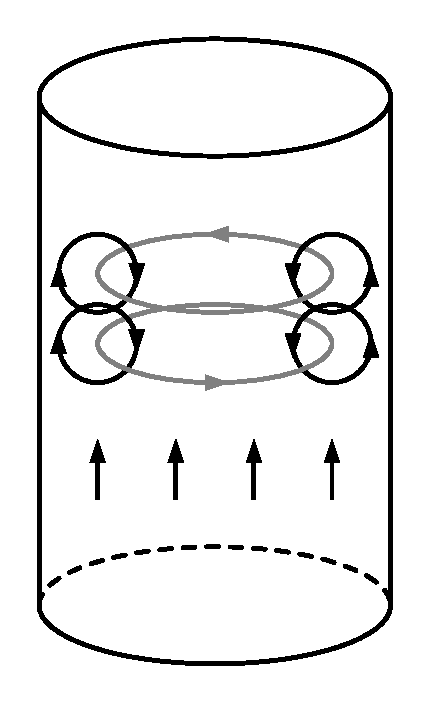
\includegraphics[width=\unitlength,page=1]{res/Skineffect_reason.pdf}}%
    \put(0.60476562,0.46865778){\color[rgb]{0,0,0}\makebox(0,0)[lt]{\lineheight{3}\smash{\begin{tabular}[t]{l}\LARGE$I$\end{tabular}}}}%
    \put(0.76026257,1.12400698){\color[rgb]{0,0,0}\makebox(0,0)[lt]{\lineheight{3}\smash{\begin{tabular}[t]{l}\LARGE$I_W$\end{tabular}}}}%
    \put(0.47817197,1.13326161){\color[rgb]{0.50196078,0.50196078,0.50196078}\makebox(0,0)[lt]{\lineheight{3}\smash{\begin{tabular}[t]{l}\LARGE$\vec{H}$\end{tabular}}}}%
  \end{picture}%
\endgroup%
}\hspace{1cm}
		  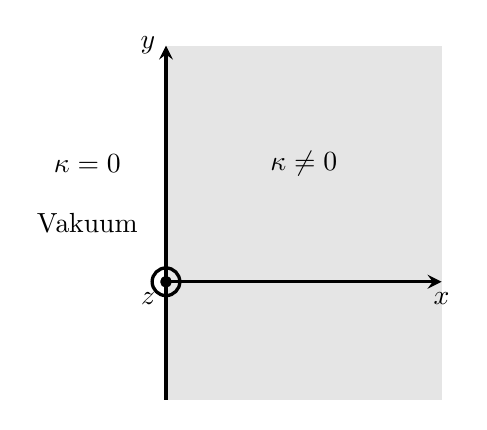
\begin{tikzpicture}[line width = 1.2pt, line join=round,x=1cm,y=1cm,>=stealth]
	% Schatten für den Stoff
	\fill [color = lightgray!40] (0,3) rectangle (3.5,-1.5);
	% Koordinatensystem
	\draw [->] (0,0) -- (3.5,0) node [anchor = north] {$ x $};
	\draw [->] (0,-1.5) -- (0,3) node [anchor = east] {$ y $};
	\filldraw (0,0) circle (1.5pt);
	\draw (0,0) circle (5pt);
	\draw (0,0) node [anchor = north east] {$ z $};
	% Leitfähigkeiten
	\draw (1.75,1.5) node {$ \kappa \neq 0 $};
	\draw (-1,1.5) node {$ \kappa = 0 $};
	\draw (-1,0.75) node {Vakuum};
\end{tikzpicture}
	  \end{center}
		  Im Folgenden soll untersucht werden, wie tief Felder in einen Leiter eindringen. Wie genau die Anregung erfolgt, ist dabei nicht von Interesse. Technisch würde man bspw. eine Quelle anlegen. Betrachtet werden zwei unendlich ausgedehnte Halbräume (wie im rechten Bild), auf der linken Seite ein Vakuum, auf der rechten Seite ein Leiter. Aufgrund der Geometrie der Anordnung gibt es Translationsinvarianz in $y$ und $z$- Richtung. \(\vec{E} \) und \(\vec{B}  \) sind also unabhängig von \(y\) und \(z\), dementsprechend sind auch die  Ableitungen nach \(y\) und \(z\) Null:
		        \begin{equation}\label{transin}
			        \dfrac{\partial}{\partial y} = \dfrac{\partial}{\partial z} = 0
		        \end{equation}
		   Das Lösungsgebiet ist $x\geq0$, also im Leiter. Es wird eine harmonische Zeitabhängigkeit vorausgesetzt, weshalb $\frac{\partial}{\partial t}$ zu $\mathrm{j}\omega$ mit einer einzigen Frequenz $\omega$ wird. Zunächst kann man noch einmal die Diffusionsgleichungen (Transformation von \ref{diffE} und \ref{diffB} in den Bildbereich, Beachtung der Translationsinvarianz) aufschreiben:
	  \begin{align*}
		  \Delta \ubar{\vec{E}}                           & = \mathrm{j}\omega\mu\kappa \ubar{\vec{E}}  & \Delta \vec{\ubar{B}}                           & = \mathrm{j}\omega\mu \kappa \vec{\ubar{B}}  \\
		  \dfrac{\partial^2}{\partial x^2} \ubar{\vec{E}} & = \mathrm{j}\omega\mu \kappa \ubar{\vec{E}} & \dfrac{\partial^2}{\partial x^2} \vec{\ubar{B}} & = \mathrm{j}\omega \mu \kappa \vec{\ubar{B}} \\
		  \ubar{\vec{E}}                                  & = \sum_{i=x,y,z}\ubar{E}_i \vu{i}           & \vec{\ubar{B}}                                  & = \sum_{i=x,y,z}\ubar{B}_i \vu{i}
	  \end{align*}
			   Aufgrund von \ref{transin} hat die Rotation des E-Feldes hat keine $x$-Komponente. Es gilt mit \ref{LeviCita} und Summenkonvention:
			        \begin{equation}\begin{split}
					        \rot \ubar{\vec{E}} = \varepsilon_{ijk} \vu{i} \partial_j\ubar{E}_k \stackrel{\text{hier}}{=} -\partial_x\ubar{E}_z \vec{e_y} + \partial_x\ubar{E}_y \vec{e_z} \stackrel{!}{=} -\mathrm{j}\omega   \sum_{i=x,y,z}\ubar{B}_i \vu{i} \implies \boxed{\ubar{B}_x=0}
				        \end{split}\end{equation}
			   Analog kann man für $B$ vorgehen:
			        \begin{equation}\begin{split}
					        \mu^{-1} \rot \vec{\ubar{B}} = \rot \vec{\ubar{H}} = \ubar{\vec{J}} = \kappa\ubar{\vec{E}} \implies \boxed{\ubar{E}_x=0}
				        \end{split}\end{equation}
			        Es folgt also, dass sowohl das B-Feld, als auch das E-Feld keine $x$-Komponente haben. Hiermit folgen 4 strukturgleiche skalare Diffusionsgleichungen
			        \begin{align}
				        \dfrac{\partial^2}{\partial x^2} \ubar{E}_y & = \mathrm{j}\omega \mu \kappa \ubar{E}_y & \dfrac{\partial^2}{\partial x^2} \ubar{B}_y & = \mathrm{j}\omega \mu \kappa \ubar{B}_y \\
				        \dfrac{\partial^2}{\partial x^2} \ubar{E}_z & = \mathrm{j}\omega \mu \kappa \ubar{E}_z & \dfrac{\partial^2}{\partial x^2} \ubar{B}_z & = \mathrm{j}\omega \mu \kappa \ubar{B}_z
			        \end{align}
			    Sowohl $y-$ als auch $z-$Komponente des elektrischen Feldes sind Tangentialkomponenten bezüglich der Grenzfläche zwischen Leiter und Vakuum. Die Tangentialkomponenten sind nach \ref{tanE} stetig, eine Normalkomponente gibt es wegen $\ubar{E}_x=0$ nicht. Es ist zweckmäßig das Koordinatensystem so zu drehen, dass $\vec{e_y} \parallel \ubar{\vec{J}}(x=0) = \kappa\ubar{\vec{E}}(x=0)$, sodass auch $\ubar{E}_z(x=0)=0$. Das funktioniert, weil es eine Translationsinvarianz in $y-$ und $z-$Richtung gibt, also $\vec{E}$ an jeder Stelle in der $y-z-$Ebene in die selbe Richtung zeigt.\\
			    Es reicht somit, eine der Gleichungen für $B$ und $E$ zu betrachten, also $\dfrac{\partial^2}{\partial x^2} \ubar{E}_y = \mathrm{j}\omega \mu \kappa \ubar{E}_y$, wobei sich $y$ nun auf das gedrehte Koordinatensystem bezieht. Die zu lösende Differentialgleichung ist eine (komplexe) homogene Differentialgleichung mit konstanten Koeffizienten, die mit dem Ansatz \ref{Fund} gelöst wird (hier: $\lambda\leftrightarrow k$). Angesetzt wird also 
			   $$\ubar{E}_\mathrm{y} = \underline{A}  \mathrm{e}^{k x} \text{ mit } [k] = \mathrm{\frac{1}{m}}$$
		   Dies liefert $k^2 = \mathrm{j}\omega \mu \kappa$, womit folgt:
		        $$
			        k_{1/2} = \pm \dfrac{1 + \mathrm{j}}{\sqrt{2}} \sqrt{\omega \mu \kappa}
			        = \pm \left( 1 + \mathrm{j}\right) \sqrt{\dfrac{\omega \mu \kappa}{2}}
			        := \pm \dfrac{1 + \mathrm{j}}{\delta}
		        $$
		   Hierbei wird $\delta$ als die \textbf{Eindringtiefe} bzw. \textbf{Skin-Tiefe} definiert, es handelt sich um eine charakteristische Länge:
		        \begin{equation}
		        	 \boxed{ \delta = \sqrt{\dfrac{2}{\omega \mu \kappa}} } \quad [\delta] =\mathrm{m}
		        \end{equation}		        
		  Die allgemeine Lösung ist somit
		        \begin{equation}
			        \boxed{\ubar{E}_\mathrm{y} = \underline{A}_1  \mathrm{e}^{\frac{x}{\delta}}  \mathrm{e}^{\mathrm{j}\frac{x}{\delta}} + \underline{A}_2   \mathrm{e}^{-\frac{x}{\delta}}  \mathrm{e}^{-\mathrm{j}\frac{x}{\delta}} }
		        \end{equation}
		Diese Gleichung kann man analog (Konstanten bekommen einen $'$, um Verwechslungen vorzubeugen) für $\ubar{E}_z$ schreiben und daraus schlussfolgern, dass sich die bisher getroffene Vereinbarung $\ubar{E}_z(x=0)$ auf den gesamten Raum erstrecken muss. Die einzige Möglichkeit, dass $\ubar{E}_z(x=0)=0$ gilt, ist, dass $\ubar{A'}_1=\ubar{A'}_2=0$. $\ubar{A'}_1=-\ubar{A'}_2\neq0$ hätte im Unendlichen das Problem, dass das elektrische Feld divergiert.  Mit \ref{ggmqs4} folgt nun:
		 \begin{equation}\label{identBE}\rot \ubar{\vec{E}} = \varepsilon_{ijk} \vu{i} \partial_j\ubar{E}_k = \textcolor{green}{-\partial_x\ubar{E}_z \vec{e_y}} + \textcolor{red}{\partial_x\ubar{E}_y \vec{e_z}} = -\mathrm{j}\omega   \sum_{i=x,\textcolor{green}{y},\textcolor{red}{z}}\ubar{B}_i \vu{i}
		 \end{equation}
		  Wegen der Festlegung $\ubar{E}_z=0$ folgt also unmittelbar $\ubar{B}_y=0$, $B$  und $E$ stehen also orthogonal zueinander. Man könnte nun also die Lösung für $\ubar{B}_z$ vollkommen analog zu der für $\ubar{E}_y$ hinschreiben. Einfacher ist es aber direkt mit der gefundenen Identität aus \ref{identBE} weiterzurechnen:
			        \begin{align}
				        \dfrac{\partial}{\partial x} \ubar{E}_y & = -\mathrm{j}\omega\ubar{B}_\mathrm{z} & \Rightarrow \ubar{B}_z & = -\dfrac{1}{\mathrm{j}\omega} \dfrac{\partial}{\partial x} \ubar{E}_y                                                                                                                                                                                               \nonumber\\
				                                                &                                        &                        & = -\dfrac{1 + \mathrm{j}}{\mathrm{j}\omega}  \dfrac{1}{\delta}  \left[ \underline{A}_1   \mathrm{e}^{\frac{x}{\delta}}   \mathrm{e}^{\mathrm{j}\frac{x}{\delta}} - \underline{A}_2  \mathrm{e}^{-\frac{x}{\delta}}  \mathrm{e}^{-\mathrm{j}\frac{x}{\delta}} \right]
			        \end{align}
			  Nun müssen die Konstanten bestimmt werden:
			        \begin{enumerate}
				        \item Für \(x \,\rightarrow\, \infty \)  darf das E-Feld nicht divergieren $\Rightarrow$
				              $\boxed{\underline{A}_1 = 0}$
				        \item Bei \(x = 0 \) gilt $\ubar{E}_{y} = \ubar{E}_{y}(x = 0) = \frac{1}{\kappa}\ubar{J}_y(x=0)=\ubar{E}_{y0} =\frac{1}{\kappa}\ubar{J}_{y0}  \Rightarrow \boxed{\underline{A}_2 = \ubar{E}_{y0}}$
			        \end{enumerate}
			  Somit folgt:
			        \begin{align}
				        \ubar{E}_{y} & = \ubar{E}_{y0}  \mathrm{e}^{-\frac{x}{\delta}}  \mathrm{e}^{-\mathrm{j}\frac{x}{\delta}} & \ubar{H}_\mathrm{z} & = \dfrac{\ubar{B}_\mathrm{z}}{\mu} = \dfrac{1 + \mathrm{j}}{\mathrm{j}\omega\mu} \dfrac{1}{\delta} \ubar{E}_{y0}  \mathrm{e}^{-\frac{x}{\delta}}  \mathrm{e}^{-\mathrm{j}\frac{x}{\delta}} & \delta & = \sqrt{\dfrac{2}{\omega \mu \kappa}}
			        \end{align}
			        Wird $\ubar{E}_{y0}$ als elektrisches Feld an der Oberfläche vorgegeben (die konkrete Ursache für dieses Feld ist weiterhin nicht von Belang, es geht nur darum wie tief das Feld in den Leiter eindringt), so kann man beobachten, dass bei unendlichem $\kappa/\omega/\mu$ das Feld wegen der gegen 0 strebenden Skin-Tiefe gar nicht in das Medium eindringt. Nun wird umgestellt, dabei werden die Begriffe \textbf{Dämpfung} und \textbf{Phasendrehung} eingeführt:
			        \begin{equation}\begin{split}
					        \ubar{H}_z &= \dfrac{1 - \mathrm{j}}{\omega \delta \mu} \ubar{E}_{y0}  \mathrm{e}^{-\frac{x}{\delta}}  \mathrm{e}^{-\mathrm{j}\frac{x}{\delta}} \\
					        &= \left(1 - \mathrm{j}\right) \sqrt{\dfrac{\kappa}{2 \omega \mu}}  \ubar{E}_{y0}  \mathrm{e}^{-\frac{x}{\delta}}  \mathrm{e}^{-\mathrm{j}\frac{x}{\delta}} \\
					        &= \dfrac{\kappa \delta}{2} \underbrace{\left( 1 - \mathrm{j}\right)}_{\sqrt{2} \mathrm{e}^{-\mathrm{j}\frac{\pi}{4}}} \ubar{E}_{y0} \underbrace{ \mathrm{e}^{-\frac{x}{\delta}}}_{\text{Dämpfung}} \underbrace{ \mathrm{e}^{-\mathrm{j}\frac{x}{\delta}}}_{\substack{\text{Phasen-}\\ \text{drehung}}} = \underbrace{\kappa \ubar{E}_{y0}}_{\ubar{J}_{y0}}\dfrac{\delta}{\sqrt{2}}  \mathrm{e}^{-\frac{x}{\delta}}  \mathrm{e}^{-\mathrm{j}\frac{x}{\delta}} \mathrm{e}^{-\mathrm{j}\frac{\pi}{4}}
				        \end{split}\end{equation}
			        Die finale Lösung für $x\ge 0$ (\textbf{im Leiter}) lautet also:
			        \begin{align}\label{finalskin}
			        	\ubar{\vec{E}} = \ubar{E}_{y}\vec{e_y}                             & = \ubar{E}_{y0}  \mathrm{e}^{-\frac{x}{\delta}}  \mathrm{e}^{-\mathrm{j}\frac{x}{\delta}}\vec{e_y}        & \vec{\ubar{H}} =\ubar{H}_{z}\vec{e_z} & = \kappa \ubar{E}_{y0}\dfrac{\delta}{\sqrt{2}}  \mathrm{e}^{-\frac{x}{\delta}}  \mathrm{e}^{-\mathrm{j}\frac{x}{\delta}} \mathrm{e}^{-\mathrm{j}\frac{\pi}{4}}\vec{e_z} \\
			        	\ubar{\vec{J}} = \ubar{J}_{y}\vec{e_y}=\kappa\ubar{E}_{y}\vec{e_y} & = \kappa \ubar{E}_{y0}  \mathrm{e}^{-\frac{x}{\delta}}  \mathrm{e}^{-\mathrm{j}\frac{x}{\delta}}\vec{e_y} & \delta                                & = \sqrt{\dfrac{2}{\omega \mu \kappa}}\nonumber
			        \end{align}
			  Es gilt: $\frac{\left| \ubar{H}_{z}(x = \delta) \right|}{\left| \ubar{H}_{z}(x = 0) \right|} = \frac{\left| \ubar{E}_{y}(x = \delta) \right|}{\left| \ubar{E}_{y}(x = 0) \right|}=  \mathrm{e}^{-1} \approx 0,37$; nach $2\delta$: $ \mathrm{e}^{-2} \approx 0,14$ usw. Beim Übergang in den Zeitbereich ist klar, dass das E- und H-Feld harmonisch schwingen, wobei das H-Feld gegenüber dem E-Feld eine Phasendrehung von $\frac{\pi}{4}$ hat (das erklärt den Offset zwischen blauer und roter Kurve). 
\begin{center}
		  \begin{minipage}{\textwidth}
			  \centering
			  \resizebox{.8\textwidth}{!}{%% Creator: Matplotlib, PGF backend
%%
%% To include the figure in your LaTeX document, write
%%   \input{<filename>.pgf}
%%
%% Make sure the required packages are loaded in your preamble
%%   \usepackage{pgf}
%%
%% Also ensure that all the required font packages are loaded; for instance,
%% the lmodern package is sometimes necessary when using math font.
%%   \usepackage{lmodern}
%%
%% Figures using additional raster images can only be included by \input if
%% they are in the same directory as the main LaTeX file. For loading figures
%% from other directories you can use the `import` package
%%   \usepackage{import}
%%
%% and then include the figures with
%%   \import{<path to file>}{<filename>.pgf}
%%
%% Matplotlib used the following preamble
%%   
%%   \usepackage{fontspec}
%%   \setmainfont{DejaVuSerif.ttf}[Path=\detokenize{/home/henning/.local/lib/python3.10/site-packages/matplotlib/mpl-data/fonts/ttf/}]
%%   \setsansfont{DejaVuSans.ttf}[Path=\detokenize{/home/henning/.local/lib/python3.10/site-packages/matplotlib/mpl-data/fonts/ttf/}]
%%   \setmonofont{DejaVuSansMono.ttf}[Path=\detokenize{/home/henning/.local/lib/python3.10/site-packages/matplotlib/mpl-data/fonts/ttf/}]
%%   \makeatletter\@ifpackageloaded{underscore}{}{\usepackage[strings]{underscore}}\makeatother
%%
\begingroup%
\makeatletter%
\begin{pgfpicture}%
\pgfpathrectangle{\pgfpointorigin}{\pgfqpoint{7.115308in}{4.436417in}}%
\pgfusepath{use as bounding box, clip}%
\begin{pgfscope}%
\pgfsetbuttcap%
\pgfsetmiterjoin%
\pgfsetlinewidth{0.000000pt}%
\definecolor{currentstroke}{rgb}{0.000000,0.000000,0.000000}%
\pgfsetstrokecolor{currentstroke}%
\pgfsetstrokeopacity{0.000000}%
\pgfsetdash{}{0pt}%
\pgfpathmoveto{\pgfqpoint{0.000000in}{-0.000000in}}%
\pgfpathlineto{\pgfqpoint{7.115308in}{-0.000000in}}%
\pgfpathlineto{\pgfqpoint{7.115308in}{4.436417in}}%
\pgfpathlineto{\pgfqpoint{0.000000in}{4.436417in}}%
\pgfpathlineto{\pgfqpoint{0.000000in}{-0.000000in}}%
\pgfpathclose%
\pgfusepath{}%
\end{pgfscope}%
\begin{pgfscope}%
\pgfsetbuttcap%
\pgfsetmiterjoin%
\pgfsetlinewidth{0.000000pt}%
\definecolor{currentstroke}{rgb}{0.000000,0.000000,0.000000}%
\pgfsetstrokecolor{currentstroke}%
\pgfsetstrokeopacity{0.000000}%
\pgfsetdash{}{0pt}%
\pgfpathmoveto{\pgfqpoint{0.815308in}{0.526079in}}%
\pgfpathlineto{\pgfqpoint{7.015308in}{0.526079in}}%
\pgfpathlineto{\pgfqpoint{7.015308in}{4.283655in}}%
\pgfpathlineto{\pgfqpoint{0.815308in}{4.283655in}}%
\pgfpathlineto{\pgfqpoint{0.815308in}{0.526079in}}%
\pgfpathclose%
\pgfusepath{}%
\end{pgfscope}%
\begin{pgfscope}%
\pgfpathrectangle{\pgfqpoint{0.815308in}{0.526079in}}{\pgfqpoint{6.200000in}{3.757576in}}%
\pgfusepath{clip}%
\pgfsetrectcap%
\pgfsetroundjoin%
\pgfsetlinewidth{0.803000pt}%
\definecolor{currentstroke}{rgb}{0.690196,0.690196,0.690196}%
\pgfsetstrokecolor{currentstroke}%
\pgfsetdash{}{0pt}%
\pgfpathmoveto{\pgfqpoint{1.097126in}{0.526079in}}%
\pgfpathlineto{\pgfqpoint{1.097126in}{4.283655in}}%
\pgfusepath{stroke}%
\end{pgfscope}%
\begin{pgfscope}%
\pgfsetbuttcap%
\pgfsetroundjoin%
\definecolor{currentfill}{rgb}{0.000000,0.000000,0.000000}%
\pgfsetfillcolor{currentfill}%
\pgfsetlinewidth{0.803000pt}%
\definecolor{currentstroke}{rgb}{0.000000,0.000000,0.000000}%
\pgfsetstrokecolor{currentstroke}%
\pgfsetdash{}{0pt}%
\pgfsys@defobject{currentmarker}{\pgfqpoint{0.000000in}{-0.048611in}}{\pgfqpoint{0.000000in}{0.000000in}}{%
\pgfpathmoveto{\pgfqpoint{0.000000in}{0.000000in}}%
\pgfpathlineto{\pgfqpoint{0.000000in}{-0.048611in}}%
\pgfusepath{stroke,fill}%
}%
\begin{pgfscope}%
\pgfsys@transformshift{1.097126in}{0.526079in}%
\pgfsys@useobject{currentmarker}{}%
\end{pgfscope}%
\end{pgfscope}%
\begin{pgfscope}%
\definecolor{textcolor}{rgb}{0.000000,0.000000,0.000000}%
\pgfsetstrokecolor{textcolor}%
\pgfsetfillcolor{textcolor}%
\pgftext[x=1.097126in,y=0.428857in,,top]{\color{textcolor}\fontsize{10.000000}{12.000000}\selectfont 0.0}%
\end{pgfscope}%
\begin{pgfscope}%
\pgfpathrectangle{\pgfqpoint{0.815308in}{0.526079in}}{\pgfqpoint{6.200000in}{3.757576in}}%
\pgfusepath{clip}%
\pgfsetrectcap%
\pgfsetroundjoin%
\pgfsetlinewidth{0.803000pt}%
\definecolor{currentstroke}{rgb}{0.690196,0.690196,0.690196}%
\pgfsetstrokecolor{currentstroke}%
\pgfsetdash{}{0pt}%
\pgfpathmoveto{\pgfqpoint{2.036520in}{0.526079in}}%
\pgfpathlineto{\pgfqpoint{2.036520in}{4.283655in}}%
\pgfusepath{stroke}%
\end{pgfscope}%
\begin{pgfscope}%
\pgfsetbuttcap%
\pgfsetroundjoin%
\definecolor{currentfill}{rgb}{0.000000,0.000000,0.000000}%
\pgfsetfillcolor{currentfill}%
\pgfsetlinewidth{0.803000pt}%
\definecolor{currentstroke}{rgb}{0.000000,0.000000,0.000000}%
\pgfsetstrokecolor{currentstroke}%
\pgfsetdash{}{0pt}%
\pgfsys@defobject{currentmarker}{\pgfqpoint{0.000000in}{-0.048611in}}{\pgfqpoint{0.000000in}{0.000000in}}{%
\pgfpathmoveto{\pgfqpoint{0.000000in}{0.000000in}}%
\pgfpathlineto{\pgfqpoint{0.000000in}{-0.048611in}}%
\pgfusepath{stroke,fill}%
}%
\begin{pgfscope}%
\pgfsys@transformshift{2.036520in}{0.526079in}%
\pgfsys@useobject{currentmarker}{}%
\end{pgfscope}%
\end{pgfscope}%
\begin{pgfscope}%
\definecolor{textcolor}{rgb}{0.000000,0.000000,0.000000}%
\pgfsetstrokecolor{textcolor}%
\pgfsetfillcolor{textcolor}%
\pgftext[x=2.036520in,y=0.428857in,,top]{\color{textcolor}\fontsize{10.000000}{12.000000}\selectfont 0.5}%
\end{pgfscope}%
\begin{pgfscope}%
\pgfpathrectangle{\pgfqpoint{0.815308in}{0.526079in}}{\pgfqpoint{6.200000in}{3.757576in}}%
\pgfusepath{clip}%
\pgfsetrectcap%
\pgfsetroundjoin%
\pgfsetlinewidth{0.803000pt}%
\definecolor{currentstroke}{rgb}{0.690196,0.690196,0.690196}%
\pgfsetstrokecolor{currentstroke}%
\pgfsetdash{}{0pt}%
\pgfpathmoveto{\pgfqpoint{2.975914in}{0.526079in}}%
\pgfpathlineto{\pgfqpoint{2.975914in}{4.283655in}}%
\pgfusepath{stroke}%
\end{pgfscope}%
\begin{pgfscope}%
\pgfsetbuttcap%
\pgfsetroundjoin%
\definecolor{currentfill}{rgb}{0.000000,0.000000,0.000000}%
\pgfsetfillcolor{currentfill}%
\pgfsetlinewidth{0.803000pt}%
\definecolor{currentstroke}{rgb}{0.000000,0.000000,0.000000}%
\pgfsetstrokecolor{currentstroke}%
\pgfsetdash{}{0pt}%
\pgfsys@defobject{currentmarker}{\pgfqpoint{0.000000in}{-0.048611in}}{\pgfqpoint{0.000000in}{0.000000in}}{%
\pgfpathmoveto{\pgfqpoint{0.000000in}{0.000000in}}%
\pgfpathlineto{\pgfqpoint{0.000000in}{-0.048611in}}%
\pgfusepath{stroke,fill}%
}%
\begin{pgfscope}%
\pgfsys@transformshift{2.975914in}{0.526079in}%
\pgfsys@useobject{currentmarker}{}%
\end{pgfscope}%
\end{pgfscope}%
\begin{pgfscope}%
\definecolor{textcolor}{rgb}{0.000000,0.000000,0.000000}%
\pgfsetstrokecolor{textcolor}%
\pgfsetfillcolor{textcolor}%
\pgftext[x=2.975914in,y=0.428857in,,top]{\color{textcolor}\fontsize{10.000000}{12.000000}\selectfont 1.0}%
\end{pgfscope}%
\begin{pgfscope}%
\pgfpathrectangle{\pgfqpoint{0.815308in}{0.526079in}}{\pgfqpoint{6.200000in}{3.757576in}}%
\pgfusepath{clip}%
\pgfsetrectcap%
\pgfsetroundjoin%
\pgfsetlinewidth{0.803000pt}%
\definecolor{currentstroke}{rgb}{0.690196,0.690196,0.690196}%
\pgfsetstrokecolor{currentstroke}%
\pgfsetdash{}{0pt}%
\pgfpathmoveto{\pgfqpoint{3.915308in}{0.526079in}}%
\pgfpathlineto{\pgfqpoint{3.915308in}{4.283655in}}%
\pgfusepath{stroke}%
\end{pgfscope}%
\begin{pgfscope}%
\pgfsetbuttcap%
\pgfsetroundjoin%
\definecolor{currentfill}{rgb}{0.000000,0.000000,0.000000}%
\pgfsetfillcolor{currentfill}%
\pgfsetlinewidth{0.803000pt}%
\definecolor{currentstroke}{rgb}{0.000000,0.000000,0.000000}%
\pgfsetstrokecolor{currentstroke}%
\pgfsetdash{}{0pt}%
\pgfsys@defobject{currentmarker}{\pgfqpoint{0.000000in}{-0.048611in}}{\pgfqpoint{0.000000in}{0.000000in}}{%
\pgfpathmoveto{\pgfqpoint{0.000000in}{0.000000in}}%
\pgfpathlineto{\pgfqpoint{0.000000in}{-0.048611in}}%
\pgfusepath{stroke,fill}%
}%
\begin{pgfscope}%
\pgfsys@transformshift{3.915308in}{0.526079in}%
\pgfsys@useobject{currentmarker}{}%
\end{pgfscope}%
\end{pgfscope}%
\begin{pgfscope}%
\definecolor{textcolor}{rgb}{0.000000,0.000000,0.000000}%
\pgfsetstrokecolor{textcolor}%
\pgfsetfillcolor{textcolor}%
\pgftext[x=3.915308in,y=0.428857in,,top]{\color{textcolor}\fontsize{10.000000}{12.000000}\selectfont 1.5}%
\end{pgfscope}%
\begin{pgfscope}%
\pgfpathrectangle{\pgfqpoint{0.815308in}{0.526079in}}{\pgfqpoint{6.200000in}{3.757576in}}%
\pgfusepath{clip}%
\pgfsetrectcap%
\pgfsetroundjoin%
\pgfsetlinewidth{0.803000pt}%
\definecolor{currentstroke}{rgb}{0.690196,0.690196,0.690196}%
\pgfsetstrokecolor{currentstroke}%
\pgfsetdash{}{0pt}%
\pgfpathmoveto{\pgfqpoint{4.854702in}{0.526079in}}%
\pgfpathlineto{\pgfqpoint{4.854702in}{4.283655in}}%
\pgfusepath{stroke}%
\end{pgfscope}%
\begin{pgfscope}%
\pgfsetbuttcap%
\pgfsetroundjoin%
\definecolor{currentfill}{rgb}{0.000000,0.000000,0.000000}%
\pgfsetfillcolor{currentfill}%
\pgfsetlinewidth{0.803000pt}%
\definecolor{currentstroke}{rgb}{0.000000,0.000000,0.000000}%
\pgfsetstrokecolor{currentstroke}%
\pgfsetdash{}{0pt}%
\pgfsys@defobject{currentmarker}{\pgfqpoint{0.000000in}{-0.048611in}}{\pgfqpoint{0.000000in}{0.000000in}}{%
\pgfpathmoveto{\pgfqpoint{0.000000in}{0.000000in}}%
\pgfpathlineto{\pgfqpoint{0.000000in}{-0.048611in}}%
\pgfusepath{stroke,fill}%
}%
\begin{pgfscope}%
\pgfsys@transformshift{4.854702in}{0.526079in}%
\pgfsys@useobject{currentmarker}{}%
\end{pgfscope}%
\end{pgfscope}%
\begin{pgfscope}%
\definecolor{textcolor}{rgb}{0.000000,0.000000,0.000000}%
\pgfsetstrokecolor{textcolor}%
\pgfsetfillcolor{textcolor}%
\pgftext[x=4.854702in,y=0.428857in,,top]{\color{textcolor}\fontsize{10.000000}{12.000000}\selectfont 2.0}%
\end{pgfscope}%
\begin{pgfscope}%
\pgfpathrectangle{\pgfqpoint{0.815308in}{0.526079in}}{\pgfqpoint{6.200000in}{3.757576in}}%
\pgfusepath{clip}%
\pgfsetrectcap%
\pgfsetroundjoin%
\pgfsetlinewidth{0.803000pt}%
\definecolor{currentstroke}{rgb}{0.690196,0.690196,0.690196}%
\pgfsetstrokecolor{currentstroke}%
\pgfsetdash{}{0pt}%
\pgfpathmoveto{\pgfqpoint{5.794096in}{0.526079in}}%
\pgfpathlineto{\pgfqpoint{5.794096in}{4.283655in}}%
\pgfusepath{stroke}%
\end{pgfscope}%
\begin{pgfscope}%
\pgfsetbuttcap%
\pgfsetroundjoin%
\definecolor{currentfill}{rgb}{0.000000,0.000000,0.000000}%
\pgfsetfillcolor{currentfill}%
\pgfsetlinewidth{0.803000pt}%
\definecolor{currentstroke}{rgb}{0.000000,0.000000,0.000000}%
\pgfsetstrokecolor{currentstroke}%
\pgfsetdash{}{0pt}%
\pgfsys@defobject{currentmarker}{\pgfqpoint{0.000000in}{-0.048611in}}{\pgfqpoint{0.000000in}{0.000000in}}{%
\pgfpathmoveto{\pgfqpoint{0.000000in}{0.000000in}}%
\pgfpathlineto{\pgfqpoint{0.000000in}{-0.048611in}}%
\pgfusepath{stroke,fill}%
}%
\begin{pgfscope}%
\pgfsys@transformshift{5.794096in}{0.526079in}%
\pgfsys@useobject{currentmarker}{}%
\end{pgfscope}%
\end{pgfscope}%
\begin{pgfscope}%
\definecolor{textcolor}{rgb}{0.000000,0.000000,0.000000}%
\pgfsetstrokecolor{textcolor}%
\pgfsetfillcolor{textcolor}%
\pgftext[x=5.794096in,y=0.428857in,,top]{\color{textcolor}\fontsize{10.000000}{12.000000}\selectfont 2.5}%
\end{pgfscope}%
\begin{pgfscope}%
\pgfpathrectangle{\pgfqpoint{0.815308in}{0.526079in}}{\pgfqpoint{6.200000in}{3.757576in}}%
\pgfusepath{clip}%
\pgfsetrectcap%
\pgfsetroundjoin%
\pgfsetlinewidth{0.803000pt}%
\definecolor{currentstroke}{rgb}{0.690196,0.690196,0.690196}%
\pgfsetstrokecolor{currentstroke}%
\pgfsetdash{}{0pt}%
\pgfpathmoveto{\pgfqpoint{6.733490in}{0.526079in}}%
\pgfpathlineto{\pgfqpoint{6.733490in}{4.283655in}}%
\pgfusepath{stroke}%
\end{pgfscope}%
\begin{pgfscope}%
\pgfsetbuttcap%
\pgfsetroundjoin%
\definecolor{currentfill}{rgb}{0.000000,0.000000,0.000000}%
\pgfsetfillcolor{currentfill}%
\pgfsetlinewidth{0.803000pt}%
\definecolor{currentstroke}{rgb}{0.000000,0.000000,0.000000}%
\pgfsetstrokecolor{currentstroke}%
\pgfsetdash{}{0pt}%
\pgfsys@defobject{currentmarker}{\pgfqpoint{0.000000in}{-0.048611in}}{\pgfqpoint{0.000000in}{0.000000in}}{%
\pgfpathmoveto{\pgfqpoint{0.000000in}{0.000000in}}%
\pgfpathlineto{\pgfqpoint{0.000000in}{-0.048611in}}%
\pgfusepath{stroke,fill}%
}%
\begin{pgfscope}%
\pgfsys@transformshift{6.733490in}{0.526079in}%
\pgfsys@useobject{currentmarker}{}%
\end{pgfscope}%
\end{pgfscope}%
\begin{pgfscope}%
\definecolor{textcolor}{rgb}{0.000000,0.000000,0.000000}%
\pgfsetstrokecolor{textcolor}%
\pgfsetfillcolor{textcolor}%
\pgftext[x=6.733490in,y=0.428857in,,top]{\color{textcolor}\fontsize{10.000000}{12.000000}\selectfont 3.0}%
\end{pgfscope}%
\begin{pgfscope}%
\definecolor{textcolor}{rgb}{0.000000,0.000000,0.000000}%
\pgfsetstrokecolor{textcolor}%
\pgfsetfillcolor{textcolor}%
\pgftext[x=3.915308in,y=0.238889in,,top]{\color{textcolor}\fontsize{10.000000}{12.000000}\selectfont \(\displaystyle x/\delta\)}%
\end{pgfscope}%
\begin{pgfscope}%
\pgfpathrectangle{\pgfqpoint{0.815308in}{0.526079in}}{\pgfqpoint{6.200000in}{3.757576in}}%
\pgfusepath{clip}%
\pgfsetrectcap%
\pgfsetroundjoin%
\pgfsetlinewidth{0.803000pt}%
\definecolor{currentstroke}{rgb}{0.690196,0.690196,0.690196}%
\pgfsetstrokecolor{currentstroke}%
\pgfsetdash{}{0pt}%
\pgfpathmoveto{\pgfqpoint{0.815308in}{0.526079in}}%
\pgfpathlineto{\pgfqpoint{7.015308in}{0.526079in}}%
\pgfusepath{stroke}%
\end{pgfscope}%
\begin{pgfscope}%
\pgfsetbuttcap%
\pgfsetroundjoin%
\definecolor{currentfill}{rgb}{0.000000,0.000000,0.000000}%
\pgfsetfillcolor{currentfill}%
\pgfsetlinewidth{0.803000pt}%
\definecolor{currentstroke}{rgb}{0.000000,0.000000,0.000000}%
\pgfsetstrokecolor{currentstroke}%
\pgfsetdash{}{0pt}%
\pgfsys@defobject{currentmarker}{\pgfqpoint{-0.048611in}{0.000000in}}{\pgfqpoint{-0.000000in}{0.000000in}}{%
\pgfpathmoveto{\pgfqpoint{-0.000000in}{0.000000in}}%
\pgfpathlineto{\pgfqpoint{-0.048611in}{0.000000in}}%
\pgfusepath{stroke,fill}%
}%
\begin{pgfscope}%
\pgfsys@transformshift{0.815308in}{0.526079in}%
\pgfsys@useobject{currentmarker}{}%
\end{pgfscope}%
\end{pgfscope}%
\begin{pgfscope}%
\definecolor{textcolor}{rgb}{0.000000,0.000000,0.000000}%
\pgfsetstrokecolor{textcolor}%
\pgfsetfillcolor{textcolor}%
\pgftext[x=0.300816in, y=0.473318in, left, base]{\color{textcolor}\fontsize{10.000000}{12.000000}\selectfont \ensuremath{-}1.00}%
\end{pgfscope}%
\begin{pgfscope}%
\pgfpathrectangle{\pgfqpoint{0.815308in}{0.526079in}}{\pgfqpoint{6.200000in}{3.757576in}}%
\pgfusepath{clip}%
\pgfsetrectcap%
\pgfsetroundjoin%
\pgfsetlinewidth{0.803000pt}%
\definecolor{currentstroke}{rgb}{0.690196,0.690196,0.690196}%
\pgfsetstrokecolor{currentstroke}%
\pgfsetdash{}{0pt}%
\pgfpathmoveto{\pgfqpoint{0.815308in}{0.995776in}}%
\pgfpathlineto{\pgfqpoint{7.015308in}{0.995776in}}%
\pgfusepath{stroke}%
\end{pgfscope}%
\begin{pgfscope}%
\pgfsetbuttcap%
\pgfsetroundjoin%
\definecolor{currentfill}{rgb}{0.000000,0.000000,0.000000}%
\pgfsetfillcolor{currentfill}%
\pgfsetlinewidth{0.803000pt}%
\definecolor{currentstroke}{rgb}{0.000000,0.000000,0.000000}%
\pgfsetstrokecolor{currentstroke}%
\pgfsetdash{}{0pt}%
\pgfsys@defobject{currentmarker}{\pgfqpoint{-0.048611in}{0.000000in}}{\pgfqpoint{-0.000000in}{0.000000in}}{%
\pgfpathmoveto{\pgfqpoint{-0.000000in}{0.000000in}}%
\pgfpathlineto{\pgfqpoint{-0.048611in}{0.000000in}}%
\pgfusepath{stroke,fill}%
}%
\begin{pgfscope}%
\pgfsys@transformshift{0.815308in}{0.995776in}%
\pgfsys@useobject{currentmarker}{}%
\end{pgfscope}%
\end{pgfscope}%
\begin{pgfscope}%
\definecolor{textcolor}{rgb}{0.000000,0.000000,0.000000}%
\pgfsetstrokecolor{textcolor}%
\pgfsetfillcolor{textcolor}%
\pgftext[x=0.300816in, y=0.943015in, left, base]{\color{textcolor}\fontsize{10.000000}{12.000000}\selectfont \ensuremath{-}0.75}%
\end{pgfscope}%
\begin{pgfscope}%
\pgfpathrectangle{\pgfqpoint{0.815308in}{0.526079in}}{\pgfqpoint{6.200000in}{3.757576in}}%
\pgfusepath{clip}%
\pgfsetrectcap%
\pgfsetroundjoin%
\pgfsetlinewidth{0.803000pt}%
\definecolor{currentstroke}{rgb}{0.690196,0.690196,0.690196}%
\pgfsetstrokecolor{currentstroke}%
\pgfsetdash{}{0pt}%
\pgfpathmoveto{\pgfqpoint{0.815308in}{1.465473in}}%
\pgfpathlineto{\pgfqpoint{7.015308in}{1.465473in}}%
\pgfusepath{stroke}%
\end{pgfscope}%
\begin{pgfscope}%
\pgfsetbuttcap%
\pgfsetroundjoin%
\definecolor{currentfill}{rgb}{0.000000,0.000000,0.000000}%
\pgfsetfillcolor{currentfill}%
\pgfsetlinewidth{0.803000pt}%
\definecolor{currentstroke}{rgb}{0.000000,0.000000,0.000000}%
\pgfsetstrokecolor{currentstroke}%
\pgfsetdash{}{0pt}%
\pgfsys@defobject{currentmarker}{\pgfqpoint{-0.048611in}{0.000000in}}{\pgfqpoint{-0.000000in}{0.000000in}}{%
\pgfpathmoveto{\pgfqpoint{-0.000000in}{0.000000in}}%
\pgfpathlineto{\pgfqpoint{-0.048611in}{0.000000in}}%
\pgfusepath{stroke,fill}%
}%
\begin{pgfscope}%
\pgfsys@transformshift{0.815308in}{1.465473in}%
\pgfsys@useobject{currentmarker}{}%
\end{pgfscope}%
\end{pgfscope}%
\begin{pgfscope}%
\definecolor{textcolor}{rgb}{0.000000,0.000000,0.000000}%
\pgfsetstrokecolor{textcolor}%
\pgfsetfillcolor{textcolor}%
\pgftext[x=0.300816in, y=1.412712in, left, base]{\color{textcolor}\fontsize{10.000000}{12.000000}\selectfont \ensuremath{-}0.50}%
\end{pgfscope}%
\begin{pgfscope}%
\pgfpathrectangle{\pgfqpoint{0.815308in}{0.526079in}}{\pgfqpoint{6.200000in}{3.757576in}}%
\pgfusepath{clip}%
\pgfsetrectcap%
\pgfsetroundjoin%
\pgfsetlinewidth{0.803000pt}%
\definecolor{currentstroke}{rgb}{0.690196,0.690196,0.690196}%
\pgfsetstrokecolor{currentstroke}%
\pgfsetdash{}{0pt}%
\pgfpathmoveto{\pgfqpoint{0.815308in}{1.935170in}}%
\pgfpathlineto{\pgfqpoint{7.015308in}{1.935170in}}%
\pgfusepath{stroke}%
\end{pgfscope}%
\begin{pgfscope}%
\pgfsetbuttcap%
\pgfsetroundjoin%
\definecolor{currentfill}{rgb}{0.000000,0.000000,0.000000}%
\pgfsetfillcolor{currentfill}%
\pgfsetlinewidth{0.803000pt}%
\definecolor{currentstroke}{rgb}{0.000000,0.000000,0.000000}%
\pgfsetstrokecolor{currentstroke}%
\pgfsetdash{}{0pt}%
\pgfsys@defobject{currentmarker}{\pgfqpoint{-0.048611in}{0.000000in}}{\pgfqpoint{-0.000000in}{0.000000in}}{%
\pgfpathmoveto{\pgfqpoint{-0.000000in}{0.000000in}}%
\pgfpathlineto{\pgfqpoint{-0.048611in}{0.000000in}}%
\pgfusepath{stroke,fill}%
}%
\begin{pgfscope}%
\pgfsys@transformshift{0.815308in}{1.935170in}%
\pgfsys@useobject{currentmarker}{}%
\end{pgfscope}%
\end{pgfscope}%
\begin{pgfscope}%
\definecolor{textcolor}{rgb}{0.000000,0.000000,0.000000}%
\pgfsetstrokecolor{textcolor}%
\pgfsetfillcolor{textcolor}%
\pgftext[x=0.300816in, y=1.882409in, left, base]{\color{textcolor}\fontsize{10.000000}{12.000000}\selectfont \ensuremath{-}0.25}%
\end{pgfscope}%
\begin{pgfscope}%
\pgfpathrectangle{\pgfqpoint{0.815308in}{0.526079in}}{\pgfqpoint{6.200000in}{3.757576in}}%
\pgfusepath{clip}%
\pgfsetrectcap%
\pgfsetroundjoin%
\pgfsetlinewidth{0.803000pt}%
\definecolor{currentstroke}{rgb}{0.690196,0.690196,0.690196}%
\pgfsetstrokecolor{currentstroke}%
\pgfsetdash{}{0pt}%
\pgfpathmoveto{\pgfqpoint{0.815308in}{2.404867in}}%
\pgfpathlineto{\pgfqpoint{7.015308in}{2.404867in}}%
\pgfusepath{stroke}%
\end{pgfscope}%
\begin{pgfscope}%
\pgfsetbuttcap%
\pgfsetroundjoin%
\definecolor{currentfill}{rgb}{0.000000,0.000000,0.000000}%
\pgfsetfillcolor{currentfill}%
\pgfsetlinewidth{0.803000pt}%
\definecolor{currentstroke}{rgb}{0.000000,0.000000,0.000000}%
\pgfsetstrokecolor{currentstroke}%
\pgfsetdash{}{0pt}%
\pgfsys@defobject{currentmarker}{\pgfqpoint{-0.048611in}{0.000000in}}{\pgfqpoint{-0.000000in}{0.000000in}}{%
\pgfpathmoveto{\pgfqpoint{-0.000000in}{0.000000in}}%
\pgfpathlineto{\pgfqpoint{-0.048611in}{0.000000in}}%
\pgfusepath{stroke,fill}%
}%
\begin{pgfscope}%
\pgfsys@transformshift{0.815308in}{2.404867in}%
\pgfsys@useobject{currentmarker}{}%
\end{pgfscope}%
\end{pgfscope}%
\begin{pgfscope}%
\definecolor{textcolor}{rgb}{0.000000,0.000000,0.000000}%
\pgfsetstrokecolor{textcolor}%
\pgfsetfillcolor{textcolor}%
\pgftext[x=0.408841in, y=2.352106in, left, base]{\color{textcolor}\fontsize{10.000000}{12.000000}\selectfont 0.00}%
\end{pgfscope}%
\begin{pgfscope}%
\pgfpathrectangle{\pgfqpoint{0.815308in}{0.526079in}}{\pgfqpoint{6.200000in}{3.757576in}}%
\pgfusepath{clip}%
\pgfsetrectcap%
\pgfsetroundjoin%
\pgfsetlinewidth{0.803000pt}%
\definecolor{currentstroke}{rgb}{0.690196,0.690196,0.690196}%
\pgfsetstrokecolor{currentstroke}%
\pgfsetdash{}{0pt}%
\pgfpathmoveto{\pgfqpoint{0.815308in}{2.874564in}}%
\pgfpathlineto{\pgfqpoint{7.015308in}{2.874564in}}%
\pgfusepath{stroke}%
\end{pgfscope}%
\begin{pgfscope}%
\pgfsetbuttcap%
\pgfsetroundjoin%
\definecolor{currentfill}{rgb}{0.000000,0.000000,0.000000}%
\pgfsetfillcolor{currentfill}%
\pgfsetlinewidth{0.803000pt}%
\definecolor{currentstroke}{rgb}{0.000000,0.000000,0.000000}%
\pgfsetstrokecolor{currentstroke}%
\pgfsetdash{}{0pt}%
\pgfsys@defobject{currentmarker}{\pgfqpoint{-0.048611in}{0.000000in}}{\pgfqpoint{-0.000000in}{0.000000in}}{%
\pgfpathmoveto{\pgfqpoint{-0.000000in}{0.000000in}}%
\pgfpathlineto{\pgfqpoint{-0.048611in}{0.000000in}}%
\pgfusepath{stroke,fill}%
}%
\begin{pgfscope}%
\pgfsys@transformshift{0.815308in}{2.874564in}%
\pgfsys@useobject{currentmarker}{}%
\end{pgfscope}%
\end{pgfscope}%
\begin{pgfscope}%
\definecolor{textcolor}{rgb}{0.000000,0.000000,0.000000}%
\pgfsetstrokecolor{textcolor}%
\pgfsetfillcolor{textcolor}%
\pgftext[x=0.408841in, y=2.821803in, left, base]{\color{textcolor}\fontsize{10.000000}{12.000000}\selectfont 0.25}%
\end{pgfscope}%
\begin{pgfscope}%
\pgfpathrectangle{\pgfqpoint{0.815308in}{0.526079in}}{\pgfqpoint{6.200000in}{3.757576in}}%
\pgfusepath{clip}%
\pgfsetrectcap%
\pgfsetroundjoin%
\pgfsetlinewidth{0.803000pt}%
\definecolor{currentstroke}{rgb}{0.690196,0.690196,0.690196}%
\pgfsetstrokecolor{currentstroke}%
\pgfsetdash{}{0pt}%
\pgfpathmoveto{\pgfqpoint{0.815308in}{3.344261in}}%
\pgfpathlineto{\pgfqpoint{7.015308in}{3.344261in}}%
\pgfusepath{stroke}%
\end{pgfscope}%
\begin{pgfscope}%
\pgfsetbuttcap%
\pgfsetroundjoin%
\definecolor{currentfill}{rgb}{0.000000,0.000000,0.000000}%
\pgfsetfillcolor{currentfill}%
\pgfsetlinewidth{0.803000pt}%
\definecolor{currentstroke}{rgb}{0.000000,0.000000,0.000000}%
\pgfsetstrokecolor{currentstroke}%
\pgfsetdash{}{0pt}%
\pgfsys@defobject{currentmarker}{\pgfqpoint{-0.048611in}{0.000000in}}{\pgfqpoint{-0.000000in}{0.000000in}}{%
\pgfpathmoveto{\pgfqpoint{-0.000000in}{0.000000in}}%
\pgfpathlineto{\pgfqpoint{-0.048611in}{0.000000in}}%
\pgfusepath{stroke,fill}%
}%
\begin{pgfscope}%
\pgfsys@transformshift{0.815308in}{3.344261in}%
\pgfsys@useobject{currentmarker}{}%
\end{pgfscope}%
\end{pgfscope}%
\begin{pgfscope}%
\definecolor{textcolor}{rgb}{0.000000,0.000000,0.000000}%
\pgfsetstrokecolor{textcolor}%
\pgfsetfillcolor{textcolor}%
\pgftext[x=0.408841in, y=3.291500in, left, base]{\color{textcolor}\fontsize{10.000000}{12.000000}\selectfont 0.50}%
\end{pgfscope}%
\begin{pgfscope}%
\pgfpathrectangle{\pgfqpoint{0.815308in}{0.526079in}}{\pgfqpoint{6.200000in}{3.757576in}}%
\pgfusepath{clip}%
\pgfsetrectcap%
\pgfsetroundjoin%
\pgfsetlinewidth{0.803000pt}%
\definecolor{currentstroke}{rgb}{0.690196,0.690196,0.690196}%
\pgfsetstrokecolor{currentstroke}%
\pgfsetdash{}{0pt}%
\pgfpathmoveto{\pgfqpoint{0.815308in}{3.813958in}}%
\pgfpathlineto{\pgfqpoint{7.015308in}{3.813958in}}%
\pgfusepath{stroke}%
\end{pgfscope}%
\begin{pgfscope}%
\pgfsetbuttcap%
\pgfsetroundjoin%
\definecolor{currentfill}{rgb}{0.000000,0.000000,0.000000}%
\pgfsetfillcolor{currentfill}%
\pgfsetlinewidth{0.803000pt}%
\definecolor{currentstroke}{rgb}{0.000000,0.000000,0.000000}%
\pgfsetstrokecolor{currentstroke}%
\pgfsetdash{}{0pt}%
\pgfsys@defobject{currentmarker}{\pgfqpoint{-0.048611in}{0.000000in}}{\pgfqpoint{-0.000000in}{0.000000in}}{%
\pgfpathmoveto{\pgfqpoint{-0.000000in}{0.000000in}}%
\pgfpathlineto{\pgfqpoint{-0.048611in}{0.000000in}}%
\pgfusepath{stroke,fill}%
}%
\begin{pgfscope}%
\pgfsys@transformshift{0.815308in}{3.813958in}%
\pgfsys@useobject{currentmarker}{}%
\end{pgfscope}%
\end{pgfscope}%
\begin{pgfscope}%
\definecolor{textcolor}{rgb}{0.000000,0.000000,0.000000}%
\pgfsetstrokecolor{textcolor}%
\pgfsetfillcolor{textcolor}%
\pgftext[x=0.408841in, y=3.761197in, left, base]{\color{textcolor}\fontsize{10.000000}{12.000000}\selectfont 0.75}%
\end{pgfscope}%
\begin{pgfscope}%
\pgfpathrectangle{\pgfqpoint{0.815308in}{0.526079in}}{\pgfqpoint{6.200000in}{3.757576in}}%
\pgfusepath{clip}%
\pgfsetrectcap%
\pgfsetroundjoin%
\pgfsetlinewidth{0.803000pt}%
\definecolor{currentstroke}{rgb}{0.690196,0.690196,0.690196}%
\pgfsetstrokecolor{currentstroke}%
\pgfsetdash{}{0pt}%
\pgfpathmoveto{\pgfqpoint{0.815308in}{4.283655in}}%
\pgfpathlineto{\pgfqpoint{7.015308in}{4.283655in}}%
\pgfusepath{stroke}%
\end{pgfscope}%
\begin{pgfscope}%
\pgfsetbuttcap%
\pgfsetroundjoin%
\definecolor{currentfill}{rgb}{0.000000,0.000000,0.000000}%
\pgfsetfillcolor{currentfill}%
\pgfsetlinewidth{0.803000pt}%
\definecolor{currentstroke}{rgb}{0.000000,0.000000,0.000000}%
\pgfsetstrokecolor{currentstroke}%
\pgfsetdash{}{0pt}%
\pgfsys@defobject{currentmarker}{\pgfqpoint{-0.048611in}{0.000000in}}{\pgfqpoint{-0.000000in}{0.000000in}}{%
\pgfpathmoveto{\pgfqpoint{-0.000000in}{0.000000in}}%
\pgfpathlineto{\pgfqpoint{-0.048611in}{0.000000in}}%
\pgfusepath{stroke,fill}%
}%
\begin{pgfscope}%
\pgfsys@transformshift{0.815308in}{4.283655in}%
\pgfsys@useobject{currentmarker}{}%
\end{pgfscope}%
\end{pgfscope}%
\begin{pgfscope}%
\definecolor{textcolor}{rgb}{0.000000,0.000000,0.000000}%
\pgfsetstrokecolor{textcolor}%
\pgfsetfillcolor{textcolor}%
\pgftext[x=0.408841in, y=4.230894in, left, base]{\color{textcolor}\fontsize{10.000000}{12.000000}\selectfont 1.00}%
\end{pgfscope}%
\begin{pgfscope}%
\definecolor{textcolor}{rgb}{0.000000,0.000000,0.000000}%
\pgfsetstrokecolor{textcolor}%
\pgfsetfillcolor{textcolor}%
\pgftext[x=0.245260in,y=2.404867in,,bottom,rotate=90.000000]{\color{textcolor}\fontsize{10.000000}{12.000000}\selectfont \(\displaystyle E_y/E_y(x=0)\) bzw. \(\displaystyle H_z/H_z(x=0)\)}%
\end{pgfscope}%
\begin{pgfscope}%
\pgfpathrectangle{\pgfqpoint{0.815308in}{0.526079in}}{\pgfqpoint{6.200000in}{3.757576in}}%
\pgfusepath{clip}%
\pgfsetrectcap%
\pgfsetroundjoin%
\pgfsetlinewidth{1.505625pt}%
\definecolor{currentstroke}{rgb}{1.000000,0.000000,0.000000}%
\pgfsetstrokecolor{currentstroke}%
\pgfsetdash{}{0pt}%
\pgfpathmoveto{\pgfqpoint{1.097126in}{4.283655in}}%
\pgfpathlineto{\pgfqpoint{1.285005in}{4.096372in}}%
\pgfpathlineto{\pgfqpoint{1.472884in}{3.912427in}}%
\pgfpathlineto{\pgfqpoint{1.660762in}{3.734543in}}%
\pgfpathlineto{\pgfqpoint{1.848641in}{3.564842in}}%
\pgfpathlineto{\pgfqpoint{2.036520in}{3.404910in}}%
\pgfpathlineto{\pgfqpoint{2.224399in}{3.255871in}}%
\pgfpathlineto{\pgfqpoint{2.412278in}{3.118449in}}%
\pgfpathlineto{\pgfqpoint{2.600156in}{2.993023in}}%
\pgfpathlineto{\pgfqpoint{2.788035in}{2.879689in}}%
\pgfpathlineto{\pgfqpoint{2.975914in}{2.778307in}}%
\pgfpathlineto{\pgfqpoint{3.163793in}{2.688544in}}%
\pgfpathlineto{\pgfqpoint{3.351672in}{2.609918in}}%
\pgfpathlineto{\pgfqpoint{3.539550in}{2.541835in}}%
\pgfpathlineto{\pgfqpoint{3.727429in}{2.483614in}}%
\pgfpathlineto{\pgfqpoint{3.915308in}{2.434521in}}%
\pgfpathlineto{\pgfqpoint{4.103187in}{2.393791in}}%
\pgfpathlineto{\pgfqpoint{4.291065in}{2.360645in}}%
\pgfpathlineto{\pgfqpoint{4.478944in}{2.334307in}}%
\pgfpathlineto{\pgfqpoint{4.666823in}{2.314020in}}%
\pgfpathlineto{\pgfqpoint{4.854702in}{2.299055in}}%
\pgfpathlineto{\pgfqpoint{5.042581in}{2.288718in}}%
\pgfpathlineto{\pgfqpoint{5.230459in}{2.282356in}}%
\pgfpathlineto{\pgfqpoint{5.418338in}{2.279364in}}%
\pgfpathlineto{\pgfqpoint{5.606217in}{2.279186in}}%
\pgfpathlineto{\pgfqpoint{5.794096in}{2.281315in}}%
\pgfpathlineto{\pgfqpoint{5.981975in}{2.285293in}}%
\pgfpathlineto{\pgfqpoint{6.169853in}{2.290715in}}%
\pgfpathlineto{\pgfqpoint{6.357732in}{2.297219in}}%
\pgfpathlineto{\pgfqpoint{6.545611in}{2.304493in}}%
\pgfpathlineto{\pgfqpoint{6.733490in}{2.312264in}}%
\pgfusepath{stroke}%
\end{pgfscope}%
\begin{pgfscope}%
\pgfpathrectangle{\pgfqpoint{0.815308in}{0.526079in}}{\pgfqpoint{6.200000in}{3.757576in}}%
\pgfusepath{clip}%
\pgfsetrectcap%
\pgfsetroundjoin%
\pgfsetlinewidth{1.505625pt}%
\definecolor{currentstroke}{rgb}{0.000000,0.000000,1.000000}%
\pgfsetstrokecolor{currentstroke}%
\pgfsetdash{}{0pt}%
\pgfpathmoveto{\pgfqpoint{1.097126in}{3.733371in}}%
\pgfpathlineto{\pgfqpoint{1.285005in}{3.480934in}}%
\pgfpathlineto{\pgfqpoint{1.472884in}{3.254783in}}%
\pgfpathlineto{\pgfqpoint{1.660762in}{3.054245in}}%
\pgfpathlineto{\pgfqpoint{1.848641in}{2.878307in}}%
\pgfpathlineto{\pgfqpoint{2.036520in}{2.725694in}}%
\pgfpathlineto{\pgfqpoint{2.224399in}{2.594938in}}%
\pgfpathlineto{\pgfqpoint{2.412278in}{2.484445in}}%
\pgfpathlineto{\pgfqpoint{2.600156in}{2.392541in}}%
\pgfpathlineto{\pgfqpoint{2.788035in}{2.317519in}}%
\pgfpathlineto{\pgfqpoint{2.975914in}{2.257677in}}%
\pgfpathlineto{\pgfqpoint{3.163793in}{2.211347in}}%
\pgfpathlineto{\pgfqpoint{3.351672in}{2.176916in}}%
\pgfpathlineto{\pgfqpoint{3.539550in}{2.152852in}}%
\pgfpathlineto{\pgfqpoint{3.727429in}{2.137711in}}%
\pgfpathlineto{\pgfqpoint{3.915308in}{2.130149in}}%
\pgfpathlineto{\pgfqpoint{4.103187in}{2.128930in}}%
\pgfpathlineto{\pgfqpoint{4.291065in}{2.132925in}}%
\pgfpathlineto{\pgfqpoint{4.478944in}{2.141117in}}%
\pgfpathlineto{\pgfqpoint{4.666823in}{2.152597in}}%
\pgfpathlineto{\pgfqpoint{4.854702in}{2.166561in}}%
\pgfpathlineto{\pgfqpoint{5.042581in}{2.182307in}}%
\pgfpathlineto{\pgfqpoint{5.230459in}{2.199226in}}%
\pgfpathlineto{\pgfqpoint{5.418338in}{2.216800in}}%
\pgfpathlineto{\pgfqpoint{5.606217in}{2.234591in}}%
\pgfpathlineto{\pgfqpoint{5.794096in}{2.252239in}}%
\pgfpathlineto{\pgfqpoint{5.981975in}{2.269450in}}%
\pgfpathlineto{\pgfqpoint{6.169853in}{2.285992in}}%
\pgfpathlineto{\pgfqpoint{6.357732in}{2.301686in}}%
\pgfpathlineto{\pgfqpoint{6.545611in}{2.316403in}}%
\pgfpathlineto{\pgfqpoint{6.733490in}{2.330053in}}%
\pgfusepath{stroke}%
\end{pgfscope}%
\begin{pgfscope}%
\pgfpathrectangle{\pgfqpoint{0.815308in}{0.526079in}}{\pgfqpoint{6.200000in}{3.757576in}}%
\pgfusepath{clip}%
\pgfsetbuttcap%
\pgfsetroundjoin%
\pgfsetlinewidth{1.505625pt}%
\definecolor{currentstroke}{rgb}{0.000000,0.000000,0.000000}%
\pgfsetstrokecolor{currentstroke}%
\pgfsetdash{{5.550000pt}{2.400000pt}}{0.000000pt}%
\pgfpathmoveto{\pgfqpoint{1.097126in}{4.283655in}}%
\pgfpathlineto{\pgfqpoint{1.285005in}{4.104865in}}%
\pgfpathlineto{\pgfqpoint{1.472884in}{3.943089in}}%
\pgfpathlineto{\pgfqpoint{1.660762in}{3.796708in}}%
\pgfpathlineto{\pgfqpoint{1.848641in}{3.664257in}}%
\pgfpathlineto{\pgfqpoint{2.036520in}{3.544410in}}%
\pgfpathlineto{\pgfqpoint{2.224399in}{3.435968in}}%
\pgfpathlineto{\pgfqpoint{2.412278in}{3.337846in}}%
\pgfpathlineto{\pgfqpoint{2.600156in}{3.249061in}}%
\pgfpathlineto{\pgfqpoint{2.788035in}{3.168725in}}%
\pgfpathlineto{\pgfqpoint{2.975914in}{3.096035in}}%
\pgfpathlineto{\pgfqpoint{3.163793in}{3.030261in}}%
\pgfpathlineto{\pgfqpoint{3.351672in}{2.970747in}}%
\pgfpathlineto{\pgfqpoint{3.539550in}{2.916897in}}%
\pgfpathlineto{\pgfqpoint{3.727429in}{2.868171in}}%
\pgfpathlineto{\pgfqpoint{3.915308in}{2.824082in}}%
\pgfpathlineto{\pgfqpoint{4.103187in}{2.784188in}}%
\pgfpathlineto{\pgfqpoint{4.291065in}{2.748091in}}%
\pgfpathlineto{\pgfqpoint{4.478944in}{2.715429in}}%
\pgfpathlineto{\pgfqpoint{4.666823in}{2.685875in}}%
\pgfpathlineto{\pgfqpoint{4.854702in}{2.659134in}}%
\pgfpathlineto{\pgfqpoint{5.042581in}{2.634937in}}%
\pgfpathlineto{\pgfqpoint{5.230459in}{2.613043in}}%
\pgfpathlineto{\pgfqpoint{5.418338in}{2.593232in}}%
\pgfpathlineto{\pgfqpoint{5.606217in}{2.575307in}}%
\pgfpathlineto{\pgfqpoint{5.794096in}{2.559088in}}%
\pgfpathlineto{\pgfqpoint{5.981975in}{2.544412in}}%
\pgfpathlineto{\pgfqpoint{6.169853in}{2.531132in}}%
\pgfpathlineto{\pgfqpoint{6.357732in}{2.519117in}}%
\pgfpathlineto{\pgfqpoint{6.545611in}{2.508244in}}%
\pgfpathlineto{\pgfqpoint{6.733490in}{2.498407in}}%
\pgfusepath{stroke}%
\end{pgfscope}%
\begin{pgfscope}%
\pgfpathrectangle{\pgfqpoint{0.815308in}{0.526079in}}{\pgfqpoint{6.200000in}{3.757576in}}%
\pgfusepath{clip}%
\pgfsetbuttcap%
\pgfsetroundjoin%
\pgfsetlinewidth{1.505625pt}%
\definecolor{currentstroke}{rgb}{0.000000,0.000000,0.000000}%
\pgfsetstrokecolor{currentstroke}%
\pgfsetdash{{5.550000pt}{2.400000pt}}{0.000000pt}%
\pgfpathmoveto{\pgfqpoint{1.097126in}{0.526079in}}%
\pgfpathlineto{\pgfqpoint{1.285005in}{0.704870in}}%
\pgfpathlineto{\pgfqpoint{1.472884in}{0.866646in}}%
\pgfpathlineto{\pgfqpoint{1.660762in}{1.013027in}}%
\pgfpathlineto{\pgfqpoint{1.848641in}{1.145478in}}%
\pgfpathlineto{\pgfqpoint{2.036520in}{1.265325in}}%
\pgfpathlineto{\pgfqpoint{2.224399in}{1.373767in}}%
\pgfpathlineto{\pgfqpoint{2.412278in}{1.471889in}}%
\pgfpathlineto{\pgfqpoint{2.600156in}{1.560674in}}%
\pgfpathlineto{\pgfqpoint{2.788035in}{1.641009in}}%
\pgfpathlineto{\pgfqpoint{2.975914in}{1.713700in}}%
\pgfpathlineto{\pgfqpoint{3.163793in}{1.779473in}}%
\pgfpathlineto{\pgfqpoint{3.351672in}{1.838987in}}%
\pgfpathlineto{\pgfqpoint{3.539550in}{1.892838in}}%
\pgfpathlineto{\pgfqpoint{3.727429in}{1.941564in}}%
\pgfpathlineto{\pgfqpoint{3.915308in}{1.985653in}}%
\pgfpathlineto{\pgfqpoint{4.103187in}{2.025547in}}%
\pgfpathlineto{\pgfqpoint{4.291065in}{2.061644in}}%
\pgfpathlineto{\pgfqpoint{4.478944in}{2.094306in}}%
\pgfpathlineto{\pgfqpoint{4.666823in}{2.123860in}}%
\pgfpathlineto{\pgfqpoint{4.854702in}{2.150601in}}%
\pgfpathlineto{\pgfqpoint{5.042581in}{2.174798in}}%
\pgfpathlineto{\pgfqpoint{5.230459in}{2.196692in}}%
\pgfpathlineto{\pgfqpoint{5.418338in}{2.216502in}}%
\pgfpathlineto{\pgfqpoint{5.606217in}{2.234428in}}%
\pgfpathlineto{\pgfqpoint{5.794096in}{2.250647in}}%
\pgfpathlineto{\pgfqpoint{5.981975in}{2.265323in}}%
\pgfpathlineto{\pgfqpoint{6.169853in}{2.278602in}}%
\pgfpathlineto{\pgfqpoint{6.357732in}{2.290618in}}%
\pgfpathlineto{\pgfqpoint{6.545611in}{2.301490in}}%
\pgfpathlineto{\pgfqpoint{6.733490in}{2.311328in}}%
\pgfusepath{stroke}%
\end{pgfscope}%
\begin{pgfscope}%
\pgfpathrectangle{\pgfqpoint{0.815308in}{0.526079in}}{\pgfqpoint{6.200000in}{3.757576in}}%
\pgfusepath{clip}%
\pgfsetrectcap%
\pgfsetroundjoin%
\pgfsetlinewidth{1.505625pt}%
\definecolor{currentstroke}{rgb}{1.000000,0.000000,0.000000}%
\pgfsetstrokecolor{currentstroke}%
\pgfsetdash{}{0pt}%
\pgfpathmoveto{\pgfqpoint{3.445611in}{3.813958in}}%
\pgfpathlineto{\pgfqpoint{3.821369in}{3.813958in}}%
\pgfusepath{stroke}%
\end{pgfscope}%
\begin{pgfscope}%
\pgfpathrectangle{\pgfqpoint{0.815308in}{0.526079in}}{\pgfqpoint{6.200000in}{3.757576in}}%
\pgfusepath{clip}%
\pgfsetrectcap%
\pgfsetroundjoin%
\pgfsetlinewidth{1.505625pt}%
\definecolor{currentstroke}{rgb}{0.000000,0.000000,1.000000}%
\pgfsetstrokecolor{currentstroke}%
\pgfsetdash{}{0pt}%
\pgfpathmoveto{\pgfqpoint{3.445611in}{3.813958in}}%
\pgfpathlineto{\pgfqpoint{3.711312in}{3.548258in}}%
\pgfusepath{stroke}%
\end{pgfscope}%
\begin{pgfscope}%
\pgfsetrectcap%
\pgfsetmiterjoin%
\pgfsetlinewidth{0.803000pt}%
\definecolor{currentstroke}{rgb}{0.000000,0.000000,0.000000}%
\pgfsetstrokecolor{currentstroke}%
\pgfsetdash{}{0pt}%
\pgfpathmoveto{\pgfqpoint{0.815308in}{0.526079in}}%
\pgfpathlineto{\pgfqpoint{0.815308in}{4.283655in}}%
\pgfusepath{stroke}%
\end{pgfscope}%
\begin{pgfscope}%
\pgfsetrectcap%
\pgfsetmiterjoin%
\pgfsetlinewidth{0.803000pt}%
\definecolor{currentstroke}{rgb}{0.000000,0.000000,0.000000}%
\pgfsetstrokecolor{currentstroke}%
\pgfsetdash{}{0pt}%
\pgfpathmoveto{\pgfqpoint{7.015308in}{0.526079in}}%
\pgfpathlineto{\pgfqpoint{7.015308in}{4.283655in}}%
\pgfusepath{stroke}%
\end{pgfscope}%
\begin{pgfscope}%
\pgfsetrectcap%
\pgfsetmiterjoin%
\pgfsetlinewidth{0.803000pt}%
\definecolor{currentstroke}{rgb}{0.000000,0.000000,0.000000}%
\pgfsetstrokecolor{currentstroke}%
\pgfsetdash{}{0pt}%
\pgfpathmoveto{\pgfqpoint{0.815308in}{0.526079in}}%
\pgfpathlineto{\pgfqpoint{7.015308in}{0.526079in}}%
\pgfusepath{stroke}%
\end{pgfscope}%
\begin{pgfscope}%
\pgfsetrectcap%
\pgfsetmiterjoin%
\pgfsetlinewidth{0.803000pt}%
\definecolor{currentstroke}{rgb}{0.000000,0.000000,0.000000}%
\pgfsetstrokecolor{currentstroke}%
\pgfsetdash{}{0pt}%
\pgfpathmoveto{\pgfqpoint{0.815308in}{4.283655in}}%
\pgfpathlineto{\pgfqpoint{7.015308in}{4.283655in}}%
\pgfusepath{stroke}%
\end{pgfscope}%
\begin{pgfscope}%
\pgfsetbuttcap%
\pgfsetmiterjoin%
\definecolor{currentfill}{rgb}{1.000000,1.000000,1.000000}%
\pgfsetfillcolor{currentfill}%
\pgfsetfillopacity{0.800000}%
\pgfsetlinewidth{1.003750pt}%
\definecolor{currentstroke}{rgb}{0.800000,0.800000,0.800000}%
\pgfsetstrokecolor{currentstroke}%
\pgfsetstrokeopacity{0.800000}%
\pgfsetdash{}{0pt}%
\pgfpathmoveto{\pgfqpoint{5.658958in}{3.550125in}}%
\pgfpathlineto{\pgfqpoint{6.918086in}{3.550125in}}%
\pgfpathquadraticcurveto{\pgfqpoint{6.945863in}{3.550125in}}{\pgfqpoint{6.945863in}{3.577903in}}%
\pgfpathlineto{\pgfqpoint{6.945863in}{4.186433in}}%
\pgfpathquadraticcurveto{\pgfqpoint{6.945863in}{4.214211in}}{\pgfqpoint{6.918086in}{4.214211in}}%
\pgfpathlineto{\pgfqpoint{5.658958in}{4.214211in}}%
\pgfpathquadraticcurveto{\pgfqpoint{5.631180in}{4.214211in}}{\pgfqpoint{5.631180in}{4.186433in}}%
\pgfpathlineto{\pgfqpoint{5.631180in}{3.577903in}}%
\pgfpathquadraticcurveto{\pgfqpoint{5.631180in}{3.550125in}}{\pgfqpoint{5.658958in}{3.550125in}}%
\pgfpathlineto{\pgfqpoint{5.658958in}{3.550125in}}%
\pgfpathclose%
\pgfusepath{stroke,fill}%
\end{pgfscope}%
\begin{pgfscope}%
\pgfsetrectcap%
\pgfsetroundjoin%
\pgfsetlinewidth{1.505625pt}%
\definecolor{currentstroke}{rgb}{1.000000,0.000000,0.000000}%
\pgfsetstrokecolor{currentstroke}%
\pgfsetdash{}{0pt}%
\pgfpathmoveto{\pgfqpoint{5.686735in}{4.101743in}}%
\pgfpathlineto{\pgfqpoint{5.825624in}{4.101743in}}%
\pgfpathlineto{\pgfqpoint{5.964513in}{4.101743in}}%
\pgfusepath{stroke}%
\end{pgfscope}%
\begin{pgfscope}%
\definecolor{textcolor}{rgb}{0.000000,0.000000,0.000000}%
\pgfsetstrokecolor{textcolor}%
\pgfsetfillcolor{textcolor}%
\pgftext[x=6.075624in,y=4.053132in,left,base]{\color{textcolor}\fontsize{10.000000}{12.000000}\selectfont \(\displaystyle E_y\)}%
\end{pgfscope}%
\begin{pgfscope}%
\pgfsetrectcap%
\pgfsetroundjoin%
\pgfsetlinewidth{1.505625pt}%
\definecolor{currentstroke}{rgb}{0.000000,0.000000,1.000000}%
\pgfsetstrokecolor{currentstroke}%
\pgfsetdash{}{0pt}%
\pgfpathmoveto{\pgfqpoint{5.686735in}{3.887039in}}%
\pgfpathlineto{\pgfqpoint{5.825624in}{3.887039in}}%
\pgfpathlineto{\pgfqpoint{5.964513in}{3.887039in}}%
\pgfusepath{stroke}%
\end{pgfscope}%
\begin{pgfscope}%
\definecolor{textcolor}{rgb}{0.000000,0.000000,0.000000}%
\pgfsetstrokecolor{textcolor}%
\pgfsetfillcolor{textcolor}%
\pgftext[x=6.075624in,y=3.838427in,left,base]{\color{textcolor}\fontsize{10.000000}{12.000000}\selectfont \(\displaystyle H_z\)}%
\end{pgfscope}%
\begin{pgfscope}%
\pgfsetbuttcap%
\pgfsetroundjoin%
\pgfsetlinewidth{1.505625pt}%
\definecolor{currentstroke}{rgb}{0.000000,0.000000,0.000000}%
\pgfsetstrokecolor{currentstroke}%
\pgfsetdash{{5.550000pt}{2.400000pt}}{0.000000pt}%
\pgfpathmoveto{\pgfqpoint{5.686735in}{3.683181in}}%
\pgfpathlineto{\pgfqpoint{5.825624in}{3.683181in}}%
\pgfpathlineto{\pgfqpoint{5.964513in}{3.683181in}}%
\pgfusepath{stroke}%
\end{pgfscope}%
\begin{pgfscope}%
\definecolor{textcolor}{rgb}{0.000000,0.000000,0.000000}%
\pgfsetstrokecolor{textcolor}%
\pgfsetfillcolor{textcolor}%
\pgftext[x=6.075624in,y=3.634570in,left,base]{\color{textcolor}\fontsize{10.000000}{12.000000}\selectfont Einhüllende}%
\end{pgfscope}%
\begin{pgfscope}%
\pgfsetbuttcap%
\pgfsetmiterjoin%
\definecolor{currentfill}{rgb}{0.000000,0.000000,0.000000}%
\pgfsetfillcolor{currentfill}%
\pgfsetfillopacity{0.012500}%
\pgfsetlinewidth{5.018750pt}%
\definecolor{currentstroke}{rgb}{1.000000,1.000000,1.000000}%
\pgfsetstrokecolor{currentstroke}%
\pgfsetdash{}{0pt}%
\pgfpathmoveto{\pgfqpoint{3.445611in}{3.438201in}}%
\pgfpathcurveto{\pgfqpoint{3.545263in}{3.438201in}}{\pgfqpoint{3.640847in}{3.477793in}}{\pgfqpoint{3.711312in}{3.548258in}}%
\pgfpathcurveto{\pgfqpoint{3.781776in}{3.618722in}}{\pgfqpoint{3.821369in}{3.714306in}}{\pgfqpoint{3.821369in}{3.813958in}}%
\pgfpathcurveto{\pgfqpoint{3.821369in}{3.913610in}}{\pgfqpoint{3.781776in}{4.009194in}}{\pgfqpoint{3.711312in}{4.079659in}}%
\pgfpathcurveto{\pgfqpoint{3.640847in}{4.150124in}}{\pgfqpoint{3.545263in}{4.189716in}}{\pgfqpoint{3.445611in}{4.189716in}}%
\pgfpathcurveto{\pgfqpoint{3.345959in}{4.189716in}}{\pgfqpoint{3.250375in}{4.150124in}}{\pgfqpoint{3.179910in}{4.079659in}}%
\pgfpathcurveto{\pgfqpoint{3.109446in}{4.009194in}}{\pgfqpoint{3.069853in}{3.913610in}}{\pgfqpoint{3.069853in}{3.813958in}}%
\pgfpathcurveto{\pgfqpoint{3.069853in}{3.714306in}}{\pgfqpoint{3.109446in}{3.618722in}}{\pgfqpoint{3.179910in}{3.548258in}}%
\pgfpathcurveto{\pgfqpoint{3.250375in}{3.477793in}}{\pgfqpoint{3.345959in}{3.438201in}}{\pgfqpoint{3.445611in}{3.438201in}}%
\pgfpathlineto{\pgfqpoint{3.445611in}{3.438201in}}%
\pgfpathclose%
\pgfusepath{stroke,fill}%
\end{pgfscope}%
\begin{pgfscope}%
\pgfsetbuttcap%
\pgfsetmiterjoin%
\definecolor{currentfill}{rgb}{0.000000,0.000000,0.000000}%
\pgfsetfillcolor{currentfill}%
\pgfsetfillopacity{0.012500}%
\pgfsetlinewidth{1.003750pt}%
\definecolor{currentstroke}{rgb}{0.000000,0.000000,0.000000}%
\pgfsetstrokecolor{currentstroke}%
\pgfsetdash{}{0pt}%
\pgfpathmoveto{\pgfqpoint{3.445611in}{3.438201in}}%
\pgfpathcurveto{\pgfqpoint{3.545263in}{3.438201in}}{\pgfqpoint{3.640847in}{3.477793in}}{\pgfqpoint{3.711312in}{3.548258in}}%
\pgfpathcurveto{\pgfqpoint{3.781776in}{3.618722in}}{\pgfqpoint{3.821369in}{3.714306in}}{\pgfqpoint{3.821369in}{3.813958in}}%
\pgfpathcurveto{\pgfqpoint{3.821369in}{3.913610in}}{\pgfqpoint{3.781776in}{4.009194in}}{\pgfqpoint{3.711312in}{4.079659in}}%
\pgfpathcurveto{\pgfqpoint{3.640847in}{4.150124in}}{\pgfqpoint{3.545263in}{4.189716in}}{\pgfqpoint{3.445611in}{4.189716in}}%
\pgfpathcurveto{\pgfqpoint{3.345959in}{4.189716in}}{\pgfqpoint{3.250375in}{4.150124in}}{\pgfqpoint{3.179910in}{4.079659in}}%
\pgfpathcurveto{\pgfqpoint{3.109446in}{4.009194in}}{\pgfqpoint{3.069853in}{3.913610in}}{\pgfqpoint{3.069853in}{3.813958in}}%
\pgfpathcurveto{\pgfqpoint{3.069853in}{3.714306in}}{\pgfqpoint{3.109446in}{3.618722in}}{\pgfqpoint{3.179910in}{3.548258in}}%
\pgfpathcurveto{\pgfqpoint{3.250375in}{3.477793in}}{\pgfqpoint{3.345959in}{3.438201in}}{\pgfqpoint{3.445611in}{3.438201in}}%
\pgfpathlineto{\pgfqpoint{3.445611in}{3.438201in}}%
\pgfpathclose%
\pgfusepath{stroke,fill}%
\end{pgfscope}%
\end{pgfpicture}%
\makeatother%
\endgroup%
}\\
			  Schwingung der Lösung (Animation $\nearrow$ \href{https://github.com/hgkdd/TET/tree/main/programs}{\enquote{programs}}) \label{schwingdloes}
		  \end{minipage}
		  \begin{minipage}{\textwidth}
			  \centering
			  \resizebox{.8\textwidth}{!}{%% Creator: Matplotlib, PGF backend
%%
%% To include the figure in your LaTeX document, write
%%   \input{<filename>.pgf}
%%
%% Make sure the required packages are loaded in your preamble
%%   \usepackage{pgf}
%%
%% Also ensure that all the required font packages are loaded; for instance,
%% the lmodern package is sometimes necessary when using math font.
%%   \usepackage{lmodern}
%%
%% Figures using additional raster images can only be included by \input if
%% they are in the same directory as the main LaTeX file. For loading figures
%% from other directories you can use the `import` package
%%   \usepackage{import}
%%
%% and then include the figures with
%%   \import{<path to file>}{<filename>.pgf}
%%
%% Matplotlib used the following preamble
%%   
%%   \usepackage{fontspec}
%%   \setmainfont{DejaVuSerif.ttf}[Path=\detokenize{/home/henning/.local/lib/python3.10/site-packages/matplotlib/mpl-data/fonts/ttf/}]
%%   \setsansfont{DejaVuSans.ttf}[Path=\detokenize{/home/henning/.local/lib/python3.10/site-packages/matplotlib/mpl-data/fonts/ttf/}]
%%   \setmonofont{DejaVuSansMono.ttf}[Path=\detokenize{/home/henning/.local/lib/python3.10/site-packages/matplotlib/mpl-data/fonts/ttf/}]
%%   \makeatletter\@ifpackageloaded{underscore}{}{\usepackage[strings]{underscore}}\makeatother
%%
\begingroup%
\makeatletter%
\begin{pgfpicture}%
\pgfpathrectangle{\pgfpointorigin}{\pgfqpoint{6.910851in}{5.294365in}}%
\pgfusepath{use as bounding box, clip}%
\begin{pgfscope}%
\pgfsetbuttcap%
\pgfsetmiterjoin%
\pgfsetlinewidth{0.000000pt}%
\definecolor{currentstroke}{rgb}{0.000000,0.000000,0.000000}%
\pgfsetstrokecolor{currentstroke}%
\pgfsetstrokeopacity{0.000000}%
\pgfsetdash{}{0pt}%
\pgfpathmoveto{\pgfqpoint{0.000000in}{0.000000in}}%
\pgfpathlineto{\pgfqpoint{6.910851in}{0.000000in}}%
\pgfpathlineto{\pgfqpoint{6.910851in}{5.294365in}}%
\pgfpathlineto{\pgfqpoint{0.000000in}{5.294365in}}%
\pgfpathlineto{\pgfqpoint{0.000000in}{0.000000in}}%
\pgfpathclose%
\pgfusepath{}%
\end{pgfscope}%
\begin{pgfscope}%
\pgfsetbuttcap%
\pgfsetmiterjoin%
\pgfsetlinewidth{0.000000pt}%
\definecolor{currentstroke}{rgb}{0.000000,0.000000,0.000000}%
\pgfsetstrokecolor{currentstroke}%
\pgfsetstrokeopacity{0.000000}%
\pgfsetdash{}{0pt}%
\pgfpathmoveto{\pgfqpoint{0.610851in}{0.521603in}}%
\pgfpathlineto{\pgfqpoint{6.810851in}{0.521603in}}%
\pgfpathlineto{\pgfqpoint{6.810851in}{5.141603in}}%
\pgfpathlineto{\pgfqpoint{0.610851in}{5.141603in}}%
\pgfpathlineto{\pgfqpoint{0.610851in}{0.521603in}}%
\pgfpathclose%
\pgfusepath{}%
\end{pgfscope}%
\begin{pgfscope}%
\pgfpathrectangle{\pgfqpoint{0.610851in}{0.521603in}}{\pgfqpoint{6.200000in}{4.620000in}}%
\pgfusepath{clip}%
\pgfsetrectcap%
\pgfsetroundjoin%
\pgfsetlinewidth{0.803000pt}%
\definecolor{currentstroke}{rgb}{0.690196,0.690196,0.690196}%
\pgfsetstrokecolor{currentstroke}%
\pgfsetdash{}{0pt}%
\pgfpathmoveto{\pgfqpoint{1.330408in}{0.521603in}}%
\pgfpathlineto{\pgfqpoint{1.330408in}{5.141603in}}%
\pgfusepath{stroke}%
\end{pgfscope}%
\begin{pgfscope}%
\pgfsetbuttcap%
\pgfsetroundjoin%
\definecolor{currentfill}{rgb}{0.000000,0.000000,0.000000}%
\pgfsetfillcolor{currentfill}%
\pgfsetlinewidth{0.803000pt}%
\definecolor{currentstroke}{rgb}{0.000000,0.000000,0.000000}%
\pgfsetstrokecolor{currentstroke}%
\pgfsetdash{}{0pt}%
\pgfsys@defobject{currentmarker}{\pgfqpoint{0.000000in}{-0.048611in}}{\pgfqpoint{0.000000in}{0.000000in}}{%
\pgfpathmoveto{\pgfqpoint{0.000000in}{0.000000in}}%
\pgfpathlineto{\pgfqpoint{0.000000in}{-0.048611in}}%
\pgfusepath{stroke,fill}%
}%
\begin{pgfscope}%
\pgfsys@transformshift{1.330408in}{0.521603in}%
\pgfsys@useobject{currentmarker}{}%
\end{pgfscope}%
\end{pgfscope}%
\begin{pgfscope}%
\definecolor{textcolor}{rgb}{0.000000,0.000000,0.000000}%
\pgfsetstrokecolor{textcolor}%
\pgfsetfillcolor{textcolor}%
\pgftext[x=1.330408in,y=0.424381in,,top]{\color{textcolor} \fontsize{10.000000}{12.000000}\selectfont 50}%
\end{pgfscope}%
\begin{pgfscope}%
\pgfpathrectangle{\pgfqpoint{0.610851in}{0.521603in}}{\pgfqpoint{6.200000in}{4.620000in}}%
\pgfusepath{clip}%
\pgfsetrectcap%
\pgfsetroundjoin%
\pgfsetlinewidth{0.803000pt}%
\definecolor{currentstroke}{rgb}{0.690196,0.690196,0.690196}%
\pgfsetstrokecolor{currentstroke}%
\pgfsetdash{}{0pt}%
\pgfpathmoveto{\pgfqpoint{2.145194in}{0.521603in}}%
\pgfpathlineto{\pgfqpoint{2.145194in}{5.141603in}}%
\pgfusepath{stroke}%
\end{pgfscope}%
\begin{pgfscope}%
\pgfsetbuttcap%
\pgfsetroundjoin%
\definecolor{currentfill}{rgb}{0.000000,0.000000,0.000000}%
\pgfsetfillcolor{currentfill}%
\pgfsetlinewidth{0.803000pt}%
\definecolor{currentstroke}{rgb}{0.000000,0.000000,0.000000}%
\pgfsetstrokecolor{currentstroke}%
\pgfsetdash{}{0pt}%
\pgfsys@defobject{currentmarker}{\pgfqpoint{0.000000in}{-0.048611in}}{\pgfqpoint{0.000000in}{0.000000in}}{%
\pgfpathmoveto{\pgfqpoint{0.000000in}{0.000000in}}%
\pgfpathlineto{\pgfqpoint{0.000000in}{-0.048611in}}%
\pgfusepath{stroke,fill}%
}%
\begin{pgfscope}%
\pgfsys@transformshift{2.145194in}{0.521603in}%
\pgfsys@useobject{currentmarker}{}%
\end{pgfscope}%
\end{pgfscope}%
\begin{pgfscope}%
\definecolor{textcolor}{rgb}{0.000000,0.000000,0.000000}%
\pgfsetstrokecolor{textcolor}%
\pgfsetfillcolor{textcolor}%
\pgftext[x=2.145194in,y=0.424381in,,top]{\color{textcolor} \fontsize{10.000000}{12.000000}\selectfont 1k}%
\end{pgfscope}%
\begin{pgfscope}%
\pgfpathrectangle{\pgfqpoint{0.610851in}{0.521603in}}{\pgfqpoint{6.200000in}{4.620000in}}%
\pgfusepath{clip}%
\pgfsetrectcap%
\pgfsetroundjoin%
\pgfsetlinewidth{0.803000pt}%
\definecolor{currentstroke}{rgb}{0.690196,0.690196,0.690196}%
\pgfsetstrokecolor{currentstroke}%
\pgfsetdash{}{0pt}%
\pgfpathmoveto{\pgfqpoint{4.023982in}{0.521603in}}%
\pgfpathlineto{\pgfqpoint{4.023982in}{5.141603in}}%
\pgfusepath{stroke}%
\end{pgfscope}%
\begin{pgfscope}%
\pgfsetbuttcap%
\pgfsetroundjoin%
\definecolor{currentfill}{rgb}{0.000000,0.000000,0.000000}%
\pgfsetfillcolor{currentfill}%
\pgfsetlinewidth{0.803000pt}%
\definecolor{currentstroke}{rgb}{0.000000,0.000000,0.000000}%
\pgfsetstrokecolor{currentstroke}%
\pgfsetdash{}{0pt}%
\pgfsys@defobject{currentmarker}{\pgfqpoint{0.000000in}{-0.048611in}}{\pgfqpoint{0.000000in}{0.000000in}}{%
\pgfpathmoveto{\pgfqpoint{0.000000in}{0.000000in}}%
\pgfpathlineto{\pgfqpoint{0.000000in}{-0.048611in}}%
\pgfusepath{stroke,fill}%
}%
\begin{pgfscope}%
\pgfsys@transformshift{4.023982in}{0.521603in}%
\pgfsys@useobject{currentmarker}{}%
\end{pgfscope}%
\end{pgfscope}%
\begin{pgfscope}%
\definecolor{textcolor}{rgb}{0.000000,0.000000,0.000000}%
\pgfsetstrokecolor{textcolor}%
\pgfsetfillcolor{textcolor}%
\pgftext[x=4.023982in,y=0.424381in,,top]{\color{textcolor} \fontsize{10.000000}{12.000000}\selectfont 1M}%
\end{pgfscope}%
\begin{pgfscope}%
\pgfpathrectangle{\pgfqpoint{0.610851in}{0.521603in}}{\pgfqpoint{6.200000in}{4.620000in}}%
\pgfusepath{clip}%
\pgfsetrectcap%
\pgfsetroundjoin%
\pgfsetlinewidth{0.803000pt}%
\definecolor{currentstroke}{rgb}{0.690196,0.690196,0.690196}%
\pgfsetstrokecolor{currentstroke}%
\pgfsetdash{}{0pt}%
\pgfpathmoveto{\pgfqpoint{5.902770in}{0.521603in}}%
\pgfpathlineto{\pgfqpoint{5.902770in}{5.141603in}}%
\pgfusepath{stroke}%
\end{pgfscope}%
\begin{pgfscope}%
\pgfsetbuttcap%
\pgfsetroundjoin%
\definecolor{currentfill}{rgb}{0.000000,0.000000,0.000000}%
\pgfsetfillcolor{currentfill}%
\pgfsetlinewidth{0.803000pt}%
\definecolor{currentstroke}{rgb}{0.000000,0.000000,0.000000}%
\pgfsetstrokecolor{currentstroke}%
\pgfsetdash{}{0pt}%
\pgfsys@defobject{currentmarker}{\pgfqpoint{0.000000in}{-0.048611in}}{\pgfqpoint{0.000000in}{0.000000in}}{%
\pgfpathmoveto{\pgfqpoint{0.000000in}{0.000000in}}%
\pgfpathlineto{\pgfqpoint{0.000000in}{-0.048611in}}%
\pgfusepath{stroke,fill}%
}%
\begin{pgfscope}%
\pgfsys@transformshift{5.902770in}{0.521603in}%
\pgfsys@useobject{currentmarker}{}%
\end{pgfscope}%
\end{pgfscope}%
\begin{pgfscope}%
\definecolor{textcolor}{rgb}{0.000000,0.000000,0.000000}%
\pgfsetstrokecolor{textcolor}%
\pgfsetfillcolor{textcolor}%
\pgftext[x=5.902770in,y=0.424381in,,top]{\color{textcolor} \fontsize{10.000000}{12.000000}\selectfont 1G}%
\end{pgfscope}%
\begin{pgfscope}%
\definecolor{textcolor}{rgb}{0.000000,0.000000,0.000000}%
\pgfsetstrokecolor{textcolor}%
\pgfsetfillcolor{textcolor}%
\pgftext[x=3.710851in,y=0.234413in,,top]{\color{textcolor} \fontsize{10.000000}{12.000000}\selectfont Frequenz / Hz}%
\end{pgfscope}%
\begin{pgfscope}%
\pgfpathrectangle{\pgfqpoint{0.610851in}{0.521603in}}{\pgfqpoint{6.200000in}{4.620000in}}%
\pgfusepath{clip}%
\pgfsetrectcap%
\pgfsetroundjoin%
\pgfsetlinewidth{0.803000pt}%
\definecolor{currentstroke}{rgb}{0.690196,0.690196,0.690196}%
\pgfsetstrokecolor{currentstroke}%
\pgfsetdash{}{0pt}%
\pgfpathmoveto{\pgfqpoint{0.610851in}{0.801993in}}%
\pgfpathlineto{\pgfqpoint{6.810851in}{0.801993in}}%
\pgfusepath{stroke}%
\end{pgfscope}%
\begin{pgfscope}%
\pgfsetbuttcap%
\pgfsetroundjoin%
\definecolor{currentfill}{rgb}{0.000000,0.000000,0.000000}%
\pgfsetfillcolor{currentfill}%
\pgfsetlinewidth{0.803000pt}%
\definecolor{currentstroke}{rgb}{0.000000,0.000000,0.000000}%
\pgfsetstrokecolor{currentstroke}%
\pgfsetdash{}{0pt}%
\pgfsys@defobject{currentmarker}{\pgfqpoint{-0.048611in}{0.000000in}}{\pgfqpoint{-0.000000in}{0.000000in}}{%
\pgfpathmoveto{\pgfqpoint{-0.000000in}{0.000000in}}%
\pgfpathlineto{\pgfqpoint{-0.048611in}{0.000000in}}%
\pgfusepath{stroke,fill}%
}%
\begin{pgfscope}%
\pgfsys@transformshift{0.610851in}{0.801993in}%
\pgfsys@useobject{currentmarker}{}%
\end{pgfscope}%
\end{pgfscope}%
\begin{pgfscope}%
\definecolor{textcolor}{rgb}{0.000000,0.000000,0.000000}%
\pgfsetstrokecolor{textcolor}%
\pgfsetfillcolor{textcolor}%
\pgftext[x=0.336898in, y=0.749231in, left, base]{\color{textcolor} \fontsize{10.000000}{12.000000}\selectfont 1µ}%
\end{pgfscope}%
\begin{pgfscope}%
\pgfpathrectangle{\pgfqpoint{0.610851in}{0.521603in}}{\pgfqpoint{6.200000in}{4.620000in}}%
\pgfusepath{clip}%
\pgfsetrectcap%
\pgfsetroundjoin%
\pgfsetlinewidth{0.803000pt}%
\definecolor{currentstroke}{rgb}{0.690196,0.690196,0.690196}%
\pgfsetstrokecolor{currentstroke}%
\pgfsetdash{}{0pt}%
\pgfpathmoveto{\pgfqpoint{0.610851in}{2.248530in}}%
\pgfpathlineto{\pgfqpoint{6.810851in}{2.248530in}}%
\pgfusepath{stroke}%
\end{pgfscope}%
\begin{pgfscope}%
\pgfsetbuttcap%
\pgfsetroundjoin%
\definecolor{currentfill}{rgb}{0.000000,0.000000,0.000000}%
\pgfsetfillcolor{currentfill}%
\pgfsetlinewidth{0.803000pt}%
\definecolor{currentstroke}{rgb}{0.000000,0.000000,0.000000}%
\pgfsetstrokecolor{currentstroke}%
\pgfsetdash{}{0pt}%
\pgfsys@defobject{currentmarker}{\pgfqpoint{-0.048611in}{0.000000in}}{\pgfqpoint{-0.000000in}{0.000000in}}{%
\pgfpathmoveto{\pgfqpoint{-0.000000in}{0.000000in}}%
\pgfpathlineto{\pgfqpoint{-0.048611in}{0.000000in}}%
\pgfusepath{stroke,fill}%
}%
\begin{pgfscope}%
\pgfsys@transformshift{0.610851in}{2.248530in}%
\pgfsys@useobject{currentmarker}{}%
\end{pgfscope}%
\end{pgfscope}%
\begin{pgfscope}%
\definecolor{textcolor}{rgb}{0.000000,0.000000,0.000000}%
\pgfsetstrokecolor{textcolor}%
\pgfsetfillcolor{textcolor}%
\pgftext[x=0.289968in, y=2.195768in, left, base]{\color{textcolor} \fontsize{10.000000}{12.000000}\selectfont 1m}%
\end{pgfscope}%
\begin{pgfscope}%
\pgfpathrectangle{\pgfqpoint{0.610851in}{0.521603in}}{\pgfqpoint{6.200000in}{4.620000in}}%
\pgfusepath{clip}%
\pgfsetrectcap%
\pgfsetroundjoin%
\pgfsetlinewidth{0.803000pt}%
\definecolor{currentstroke}{rgb}{0.690196,0.690196,0.690196}%
\pgfsetstrokecolor{currentstroke}%
\pgfsetdash{}{0pt}%
\pgfpathmoveto{\pgfqpoint{0.610851in}{3.695067in}}%
\pgfpathlineto{\pgfqpoint{6.810851in}{3.695067in}}%
\pgfusepath{stroke}%
\end{pgfscope}%
\begin{pgfscope}%
\pgfsetbuttcap%
\pgfsetroundjoin%
\definecolor{currentfill}{rgb}{0.000000,0.000000,0.000000}%
\pgfsetfillcolor{currentfill}%
\pgfsetlinewidth{0.803000pt}%
\definecolor{currentstroke}{rgb}{0.000000,0.000000,0.000000}%
\pgfsetstrokecolor{currentstroke}%
\pgfsetdash{}{0pt}%
\pgfsys@defobject{currentmarker}{\pgfqpoint{-0.048611in}{0.000000in}}{\pgfqpoint{-0.000000in}{0.000000in}}{%
\pgfpathmoveto{\pgfqpoint{-0.000000in}{0.000000in}}%
\pgfpathlineto{\pgfqpoint{-0.048611in}{0.000000in}}%
\pgfusepath{stroke,fill}%
}%
\begin{pgfscope}%
\pgfsys@transformshift{0.610851in}{3.695067in}%
\pgfsys@useobject{currentmarker}{}%
\end{pgfscope}%
\end{pgfscope}%
\begin{pgfscope}%
\definecolor{textcolor}{rgb}{0.000000,0.000000,0.000000}%
\pgfsetstrokecolor{textcolor}%
\pgfsetfillcolor{textcolor}%
\pgftext[x=0.425263in, y=3.642305in, left, base]{\color{textcolor} \fontsize{10.000000}{12.000000}\selectfont 1}%
\end{pgfscope}%
\begin{pgfscope}%
\pgfpathrectangle{\pgfqpoint{0.610851in}{0.521603in}}{\pgfqpoint{6.200000in}{4.620000in}}%
\pgfusepath{clip}%
\pgfsetrectcap%
\pgfsetroundjoin%
\pgfsetlinewidth{0.803000pt}%
\definecolor{currentstroke}{rgb}{0.690196,0.690196,0.690196}%
\pgfsetstrokecolor{currentstroke}%
\pgfsetdash{}{0pt}%
\pgfpathmoveto{\pgfqpoint{0.610851in}{5.141603in}}%
\pgfpathlineto{\pgfqpoint{6.810851in}{5.141603in}}%
\pgfusepath{stroke}%
\end{pgfscope}%
\begin{pgfscope}%
\pgfsetbuttcap%
\pgfsetroundjoin%
\definecolor{currentfill}{rgb}{0.000000,0.000000,0.000000}%
\pgfsetfillcolor{currentfill}%
\pgfsetlinewidth{0.803000pt}%
\definecolor{currentstroke}{rgb}{0.000000,0.000000,0.000000}%
\pgfsetstrokecolor{currentstroke}%
\pgfsetdash{}{0pt}%
\pgfsys@defobject{currentmarker}{\pgfqpoint{-0.048611in}{0.000000in}}{\pgfqpoint{-0.000000in}{0.000000in}}{%
\pgfpathmoveto{\pgfqpoint{-0.000000in}{0.000000in}}%
\pgfpathlineto{\pgfqpoint{-0.048611in}{0.000000in}}%
\pgfusepath{stroke,fill}%
}%
\begin{pgfscope}%
\pgfsys@transformshift{0.610851in}{5.141603in}%
\pgfsys@useobject{currentmarker}{}%
\end{pgfscope}%
\end{pgfscope}%
\begin{pgfscope}%
\definecolor{textcolor}{rgb}{0.000000,0.000000,0.000000}%
\pgfsetstrokecolor{textcolor}%
\pgfsetfillcolor{textcolor}%
\pgftext[x=0.344832in, y=5.088842in, left, base]{\color{textcolor} \fontsize{10.000000}{12.000000}\selectfont 1k}%
\end{pgfscope}%
\begin{pgfscope}%
\definecolor{textcolor}{rgb}{0.000000,0.000000,0.000000}%
\pgfsetstrokecolor{textcolor}%
\pgfsetfillcolor{textcolor}%
\pgftext[x=0.234413in,y=2.831603in,,bottom,rotate=90.000000]{\color{textcolor} \fontsize{10.000000}{12.000000}\selectfont Eindringtiefe / m}%
\end{pgfscope}%
\begin{pgfscope}%
\pgfpathrectangle{\pgfqpoint{0.610851in}{0.521603in}}{\pgfqpoint{6.200000in}{4.620000in}}%
\pgfusepath{clip}%
\pgfsetrectcap%
\pgfsetroundjoin%
\pgfsetlinewidth{1.505625pt}%
\definecolor{currentstroke}{rgb}{0.121569,0.466667,0.705882}%
\pgfsetstrokecolor{currentstroke}%
\pgfsetdash{}{0pt}%
\pgfpathmoveto{\pgfqpoint{0.892669in}{2.885057in}}%
\pgfpathlineto{\pgfqpoint{6.529032in}{0.715252in}}%
\pgfpathlineto{\pgfqpoint{6.529032in}{0.715252in}}%
\pgfusepath{stroke}%
\end{pgfscope}%
\begin{pgfscope}%
\pgfpathrectangle{\pgfqpoint{0.610851in}{0.521603in}}{\pgfqpoint{6.200000in}{4.620000in}}%
\pgfusepath{clip}%
\pgfsetrectcap%
\pgfsetroundjoin%
\pgfsetlinewidth{1.505625pt}%
\definecolor{currentstroke}{rgb}{1.000000,0.498039,0.054902}%
\pgfsetstrokecolor{currentstroke}%
\pgfsetdash{}{0pt}%
\pgfpathmoveto{\pgfqpoint{0.892669in}{2.929332in}}%
\pgfpathlineto{\pgfqpoint{6.529032in}{0.759527in}}%
\pgfpathlineto{\pgfqpoint{6.529032in}{0.759527in}}%
\pgfusepath{stroke}%
\end{pgfscope}%
\begin{pgfscope}%
\pgfpathrectangle{\pgfqpoint{0.610851in}{0.521603in}}{\pgfqpoint{6.200000in}{4.620000in}}%
\pgfusepath{clip}%
\pgfsetrectcap%
\pgfsetroundjoin%
\pgfsetlinewidth{1.505625pt}%
\definecolor{currentstroke}{rgb}{0.172549,0.627451,0.172549}%
\pgfsetstrokecolor{currentstroke}%
\pgfsetdash{}{0pt}%
\pgfpathmoveto{\pgfqpoint{0.892669in}{4.588224in}}%
\pgfpathlineto{\pgfqpoint{6.529032in}{2.418418in}}%
\pgfpathlineto{\pgfqpoint{6.529032in}{2.418418in}}%
\pgfusepath{stroke}%
\end{pgfscope}%
\begin{pgfscope}%
\pgfsetrectcap%
\pgfsetmiterjoin%
\pgfsetlinewidth{0.803000pt}%
\definecolor{currentstroke}{rgb}{0.000000,0.000000,0.000000}%
\pgfsetstrokecolor{currentstroke}%
\pgfsetdash{}{0pt}%
\pgfpathmoveto{\pgfqpoint{0.610851in}{0.521603in}}%
\pgfpathlineto{\pgfqpoint{0.610851in}{5.141603in}}%
\pgfusepath{stroke}%
\end{pgfscope}%
\begin{pgfscope}%
\pgfsetrectcap%
\pgfsetmiterjoin%
\pgfsetlinewidth{0.803000pt}%
\definecolor{currentstroke}{rgb}{0.000000,0.000000,0.000000}%
\pgfsetstrokecolor{currentstroke}%
\pgfsetdash{}{0pt}%
\pgfpathmoveto{\pgfqpoint{6.810851in}{0.521603in}}%
\pgfpathlineto{\pgfqpoint{6.810851in}{5.141603in}}%
\pgfusepath{stroke}%
\end{pgfscope}%
\begin{pgfscope}%
\pgfsetrectcap%
\pgfsetmiterjoin%
\pgfsetlinewidth{0.803000pt}%
\definecolor{currentstroke}{rgb}{0.000000,0.000000,0.000000}%
\pgfsetstrokecolor{currentstroke}%
\pgfsetdash{}{0pt}%
\pgfpathmoveto{\pgfqpoint{0.610851in}{0.521603in}}%
\pgfpathlineto{\pgfqpoint{6.810851in}{0.521603in}}%
\pgfusepath{stroke}%
\end{pgfscope}%
\begin{pgfscope}%
\pgfsetrectcap%
\pgfsetmiterjoin%
\pgfsetlinewidth{0.803000pt}%
\definecolor{currentstroke}{rgb}{0.000000,0.000000,0.000000}%
\pgfsetstrokecolor{currentstroke}%
\pgfsetdash{}{0pt}%
\pgfpathmoveto{\pgfqpoint{0.610851in}{5.141603in}}%
\pgfpathlineto{\pgfqpoint{6.810851in}{5.141603in}}%
\pgfusepath{stroke}%
\end{pgfscope}%
\begin{pgfscope}%
\pgfsetbuttcap%
\pgfsetmiterjoin%
\definecolor{currentfill}{rgb}{1.000000,1.000000,1.000000}%
\pgfsetfillcolor{currentfill}%
\pgfsetfillopacity{0.800000}%
\pgfsetlinewidth{1.003750pt}%
\definecolor{currentstroke}{rgb}{0.800000,0.800000,0.800000}%
\pgfsetstrokecolor{currentstroke}%
\pgfsetstrokeopacity{0.800000}%
\pgfsetdash{}{0pt}%
\pgfpathmoveto{\pgfqpoint{4.217657in}{4.418921in}}%
\pgfpathlineto{\pgfqpoint{6.713628in}{4.418921in}}%
\pgfpathquadraticcurveto{\pgfqpoint{6.741406in}{4.418921in}}{\pgfqpoint{6.741406in}{4.446698in}}%
\pgfpathlineto{\pgfqpoint{6.741406in}{5.044381in}}%
\pgfpathquadraticcurveto{\pgfqpoint{6.741406in}{5.072159in}}{\pgfqpoint{6.713628in}{5.072159in}}%
\pgfpathlineto{\pgfqpoint{4.217657in}{5.072159in}}%
\pgfpathquadraticcurveto{\pgfqpoint{4.189879in}{5.072159in}}{\pgfqpoint{4.189879in}{5.044381in}}%
\pgfpathlineto{\pgfqpoint{4.189879in}{4.446698in}}%
\pgfpathquadraticcurveto{\pgfqpoint{4.189879in}{4.418921in}}{\pgfqpoint{4.217657in}{4.418921in}}%
\pgfpathlineto{\pgfqpoint{4.217657in}{4.418921in}}%
\pgfpathclose%
\pgfusepath{stroke,fill}%
\end{pgfscope}%
\begin{pgfscope}%
\pgfsetrectcap%
\pgfsetroundjoin%
\pgfsetlinewidth{1.505625pt}%
\definecolor{currentstroke}{rgb}{0.121569,0.466667,0.705882}%
\pgfsetstrokecolor{currentstroke}%
\pgfsetdash{}{0pt}%
\pgfpathmoveto{\pgfqpoint{4.245434in}{4.959691in}}%
\pgfpathlineto{\pgfqpoint{4.384323in}{4.959691in}}%
\pgfpathlineto{\pgfqpoint{4.523212in}{4.959691in}}%
\pgfusepath{stroke}%
\end{pgfscope}%
\begin{pgfscope}%
\definecolor{textcolor}{rgb}{0.000000,0.000000,0.000000}%
\pgfsetstrokecolor{textcolor}%
\pgfsetfillcolor{textcolor}%
\pgftext[x=4.634323in,y=4.911080in,left,base]{\color{textcolor} \fontsize{10.000000}{12.000000}\selectfont Kupfer: $\kappa=5.80\cdot 10^7$S/m}%
\end{pgfscope}%
\begin{pgfscope}%
\pgfsetrectcap%
\pgfsetroundjoin%
\pgfsetlinewidth{1.505625pt}%
\definecolor{currentstroke}{rgb}{1.000000,0.498039,0.054902}%
\pgfsetstrokecolor{currentstroke}%
\pgfsetdash{}{0pt}%
\pgfpathmoveto{\pgfqpoint{4.245434in}{4.755834in}}%
\pgfpathlineto{\pgfqpoint{4.384323in}{4.755834in}}%
\pgfpathlineto{\pgfqpoint{4.523212in}{4.755834in}}%
\pgfusepath{stroke}%
\end{pgfscope}%
\begin{pgfscope}%
\definecolor{textcolor}{rgb}{0.000000,0.000000,0.000000}%
\pgfsetstrokecolor{textcolor}%
\pgfsetfillcolor{textcolor}%
\pgftext[x=4.634323in,y=4.707223in,left,base]{\color{textcolor} \fontsize{10.000000}{12.000000}\selectfont Aluminium: $\kappa=3.80\cdot 10^7$ S/m}%
\end{pgfscope}%
\begin{pgfscope}%
\pgfsetrectcap%
\pgfsetroundjoin%
\pgfsetlinewidth{1.505625pt}%
\definecolor{currentstroke}{rgb}{0.172549,0.627451,0.172549}%
\pgfsetstrokecolor{currentstroke}%
\pgfsetdash{}{0pt}%
\pgfpathmoveto{\pgfqpoint{4.245434in}{4.551977in}}%
\pgfpathlineto{\pgfqpoint{4.384323in}{4.551977in}}%
\pgfpathlineto{\pgfqpoint{4.523212in}{4.551977in}}%
\pgfusepath{stroke}%
\end{pgfscope}%
\begin{pgfscope}%
\definecolor{textcolor}{rgb}{0.000000,0.000000,0.000000}%
\pgfsetstrokecolor{textcolor}%
\pgfsetfillcolor{textcolor}%
\pgftext[x=4.634323in,y=4.503366in,left,base]{\color{textcolor} \fontsize{10.000000}{12.000000}\selectfont Seewasser: $\kappa=5.00S/m$}%
\end{pgfscope}%
\end{pgfpicture}%
\makeatother%
\endgroup%
}\\
			  Eindringtiefe
		  \end{minipage}
		  \end{center}
Die Berechnung des Magnetfeldes für $x<0$ (vor dem Leiter) erfolgt über \ref{ggmqs1} in Verbindung mit \ref{stokes}, die Grafik links soll den Integrationsweg verdeutlichen. Rechts wird der Weg erst im unendlichen geschlossen, deshalb verschwindet der Beitrag dieses Wegstückes. Weiterhin verschwindet der Beitrag der beiden horizontalen Wegstücken, da $H$ nur eine $z-$Komponente hat und entsprechend zu $\dd\vec{s}\parallel\vu{x}$ orthogonal steht. Somit wird das Wegintegral nur durch die Teilstrecke $\zeta$ bestimmt, wobei $H$ wegen der Translationsinvarianz nur von $x$ abhängt, also auf diesem Teilstück konstant ist. Auch das Flächenintegral kann man unter Nutzung der Translationsinvarianz so vereinfachen, dass in $z-$Richtung alles konstant ist, entsprechend nur mit $\zeta$ multipliziert wird. Außerdem gilt, dass im Vakuum kein Strom fließen kann, weshalb die $x$-Integration erst ab 0 erfolgt.\\
\begin{minipage}{0.5\textwidth}
			        \resizebox{.9\textwidth}{!}{%% Creator: Inkscape 1.0.2 (e86c8708, 2021-01-15), www.inkscape.org
%% PDF/EPS/PS + LaTeX output extension by Johan Engelen, 2010
%% Accompanies image file 'res/skin-H-Weg.pdf' (pdf, eps, ps)
%%
%% To include the image in your LaTeX document, write
%%   \input{<filename>.pdf_tex}
%%  instead of
%%   \includegraphics{<filename>.pdf}
%% To scale the image, write
%%   \def\svgwidth{<desired width>}
%%   \input{<filename>.pdf_tex}
%%  instead of
%%   \includegraphics[width=<desired width>]{<filename>.pdf}
%%
%% Images with a different path to the parent latex file can
%% be accessed with the `import' package (which may need to be
%% installed) using
%%   \usepackage{import}
%% in the preamble, and then including the image with
%%   \import{<path to file>}{<filename>.pdf_tex}
%% Alternatively, one can specify
%%   \graphicspath{{<path to file>/}}
%% 
%% For more information, please see info/svg-inkscape on CTAN:
%%   http://tug.ctan.org/tex-archive/info/svg-inkscape
%%
\begingroup%
\makeatletter%
\def\svgwidth{0.5\textwidth}
\providecommand\color[2][]{%
	\errmessage{(Inkscape) Color is used for the text in Inkscape, but the package 'color.sty' is not loaded}%
	\renewcommand\color[2][]{}%
}%
\providecommand\transparent[1]{%
	\errmessage{(Inkscape) Transparency is used (non-zero) for the text in Inkscape, but the package 'transparent.sty' is not loaded}%
	\renewcommand\transparent[1]{}%
}%
\providecommand\rotatebox[2]{#2}%
\newcommand*\fsize{\dimexpr\f@size pt\relax}%
\newcommand*\lineheight[1]{\fontsize{\fsize}{#1\fsize}\selectfont}%
\ifx\svgwidth\undefined%
	\setlength{\unitlength}{841.88976378bp}%
	\ifx\svgscale\undefined%
		\relax%
	\else%
		\setlength{\unitlength}{\unitlength * \real{\svgscale}}%
	\fi%
\else%
	\setlength{\unitlength}{\svgwidth}%
\fi%
\global\let\svgwidth\undefined%
\global\let\svgscale\undefined%
\makeatother%
\begin{picture}(1,0.70707071)%
	\tiny
	\lineheight{1}%
	\setlength\tabcolsep{0pt}%
	\put(0,0){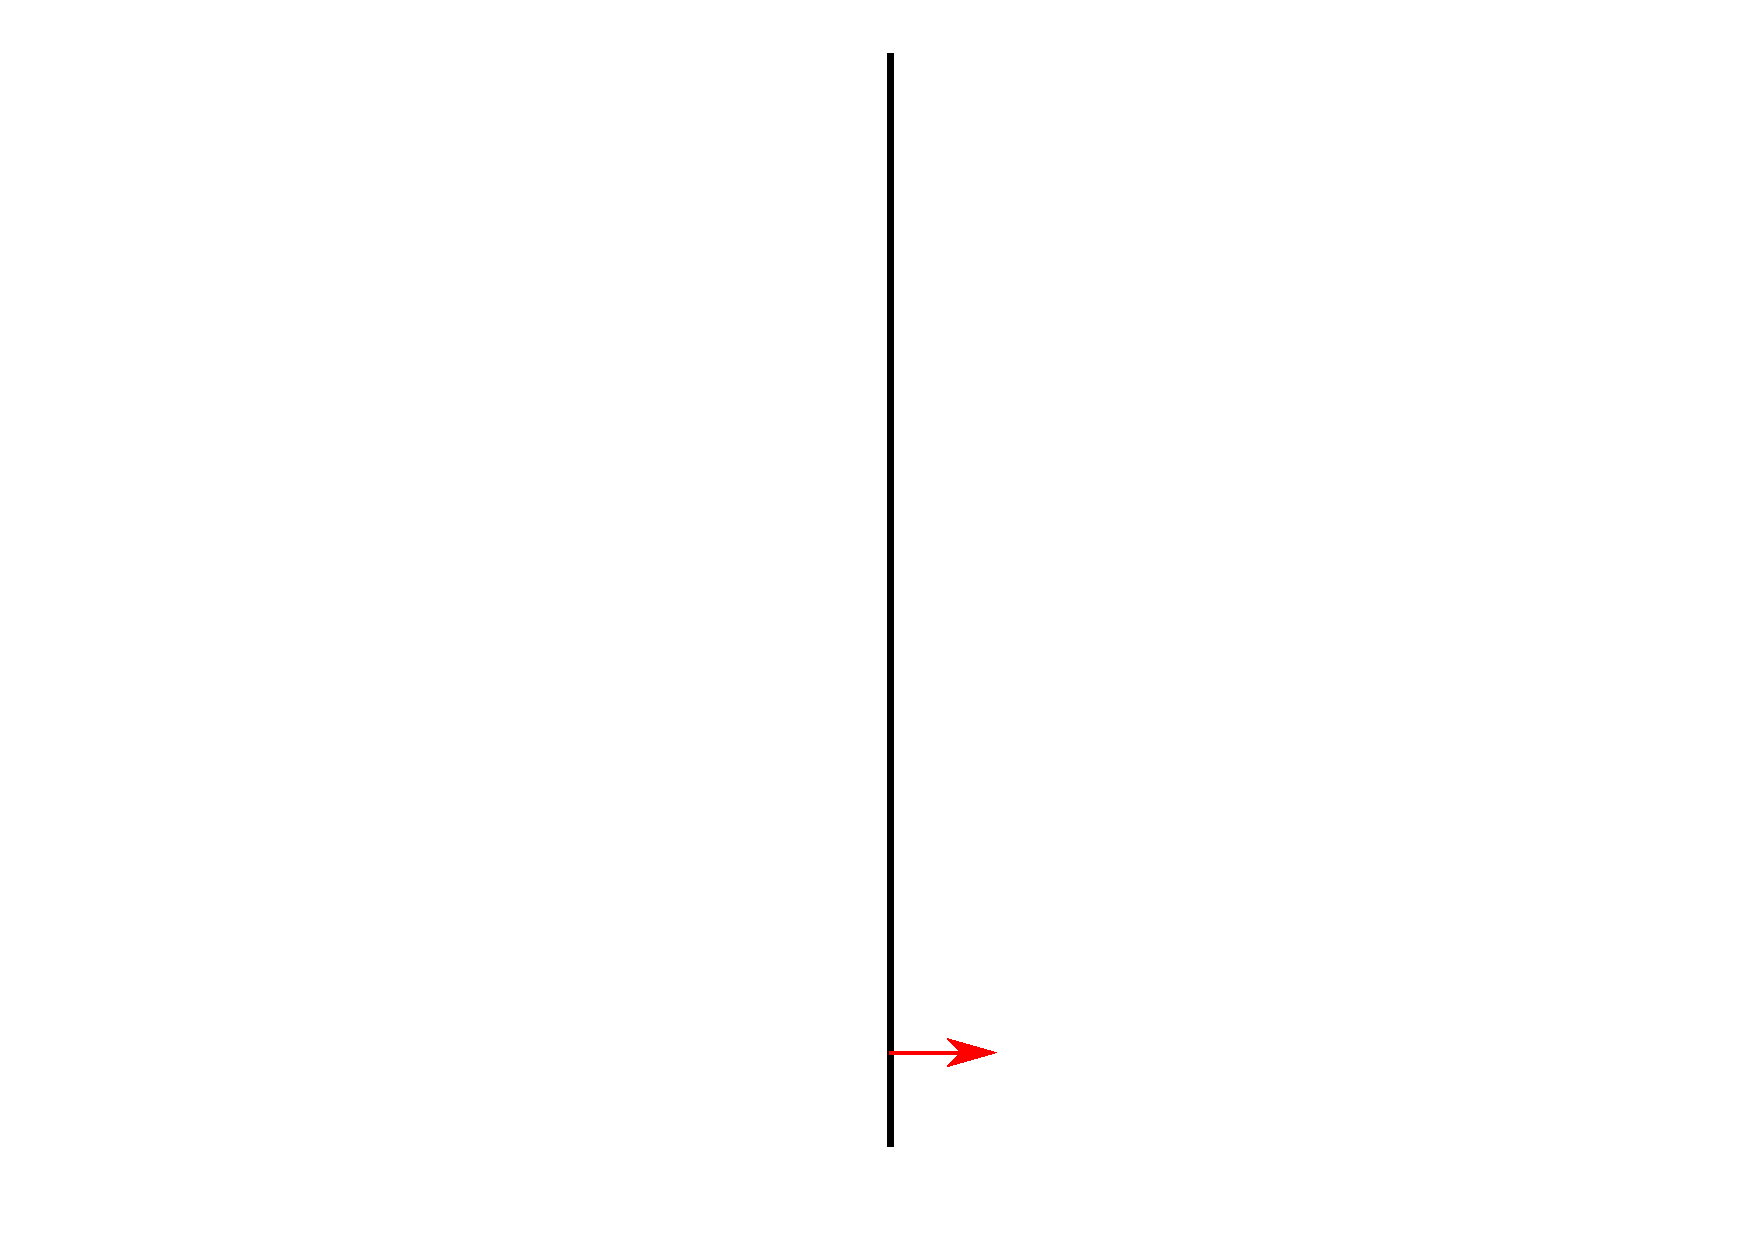
\includegraphics[width=\unitlength,page=1]{res/skin-H-Weg.pdf}}%
	\put(0.58209141,0.09491588){\color[rgb]{0.98823529,0,0}\makebox(0,0)[lt]{\lineheight{1.25}\smash{\begin{tabular}[t]{l}x\end{tabular}}}}%
	\put(0,0){\includegraphics[width=\unitlength,page=2]{res/skin-H-Weg.pdf}}%
	\put(0.46827199,0.1318683){\color[rgb]{0.98823529,0,0}\makebox(0,0)[lt]{\lineheight{1.25}\smash{\begin{tabular}[t]{l}y\end{tabular}}}}%
	\put(0.46795675,0.04442039){\color[rgb]{0.98823529,0,0}\makebox(0,0)[lt]{\lineheight{1.25}\smash{\begin{tabular}[t]{l}z\end{tabular}}}}%
	\put(0,0){\includegraphics[width=\unitlength,page=3]{res/skin-H-Weg.pdf}}%
	\put(0.3165163,0.59414568){\color[rgb]{0,0,0}\makebox(0,0)[lt]{\lineheight{1.25}\smash{\begin{tabular}[t]{l}$\kappa = 0$\end{tabular}}}}%
	\put(0.53121635,0.59414568){\color[rgb]{0,0,0}\makebox(0,0)[lt]{\lineheight{1.25}\smash{\begin{tabular}[t]{l}$\kappa \ne 0$\end{tabular}}}}%
	\put(0,0){\includegraphics[width=\unitlength,page=4]{res/skin-H-Weg.pdf}}%
	\put(0.19130244,0.39197271){\color[rgb]{0,0,0}\makebox(0,0)[lt]{\lineheight{1.25}\smash{\begin{tabular}[t]{l}$\vec{J} = \vec{0}$\end{tabular}}}}%
	\put(0.57126733,0.3923207){\color[rgb]{0,0,0}\makebox(0,0)[lt]{\lineheight{1.25}\smash{\begin{tabular}[t]{l}$\vec{J} = J_y(x) \vu{y}$\end{tabular}}}}%
	\put(0.85455836,0.20060427){\color[rgb]{0,0,0}\makebox(0,0)[lt]{\lineheight{1.25}\smash{\begin{tabular}[t]{l}$x \to \infty$\end{tabular}}}}%
	\put(0.02758345,0.39143333){\color[rgb]{0,0,0}\makebox(0,0)[lt]{\lineheight{1.25}\smash{\begin{tabular}[t]{l}$\zeta$\end{tabular}}}}%
\end{picture}%
\endgroup%
}
\end{minipage}
\begin{minipage}{0.5\textwidth}
\begin{align*}
	\oint \vec{\ubar{H}}(x)\cdot \dd\vec{s} & = \iint \ubar{\vec{J}}\cdot\dd\vec{A}                               \\
	\zeta \vec{\ubar{H}}(x)\cdot \vec{e_z}  & = \zeta \int\limits_0^\infty \ubar{\vec{J}}(x)\cdot \vec{e_y} \dd x \\
	\Aboxed{\ubar{H}_z (x<0) =\ubar{H}_z            & = (1-j) \kappa \ubar{E}_{y0} \frac{\delta}{2} = \ubar{H}_z (x=0^+)}
\end{align*}
\end{minipage}	
Es folgt also, dass $\ubar{H}_z$ im Vakuum konstant ist und das der Wert dort genau dem Wert an der Leiteroberfläche entspricht, die Tangentialkomponente des H-Feldes ist hier an der Oberfläche \textbf{stetig}. Nach \ref{tanH} gilt:
		        \begin{equation}\begin{split}
				        \vec{t}\cdot (\vec{H} _2 - \vec{H} _1) = (\vec{n} \times \vec{t})\cdot \vec{J}_A \Leftrightarrow \vec{n}\times (\vec{H} _2 - \vec{H} _1) = \vec{J}_A 
			        \end{split}\end{equation}
		   Im vorliegenden Fall kann man daraus die folgende Schlussfolgerung ziehen: 
		   \begin{equation}
		   	\vec{e_x} \times \left(\ubar{H}_z(0^+) - \ubar{H}_z(0^-)  \right) \vec{e_z} = \boxed{\vec{\ubar{J}}_A = \vec{0}}
		   \end{equation}
		   Die Tangentialkomponenten kompensieren sich also an der Oberfläche genau, weshalb die Oberflächenstromdichte verschwindet. Häufig nutzt man die \textbf{Oberflächenstromdichte} $\vec{\ubar{J}}_A$ jedoch als \textbf{Ersatzgröße} für das innere Magnetfeld $\vec{\ubar{H}}(x\ge 0)$. Die Oberflächenstromdichte ist \textbf{nicht} Stromdichte an der Oberfläche ($\nearrow$ \ref{tanH})! Setzt man $\vec{\ubar{H}}(x) = \vec{0}$ für $x\ge 0$ folgt für die Oberflächenstromdichte (sie bildet das 0 gesetzte $H$ nach):
		        \begin{equation}\begin{split}
				        \boxed{\vec{\ubar{J}}_A =\ubar{H}_z(0^-) \vec{e_y} = \int\limits_0^\infty \ubar{J}_y(x) \dd x \; \vec{e_y}}
			        \end{split}\end{equation}
		   Verwendung findet die Oberflächenstromdichte als Ersatzgröße z.B. bei numerischen Rechnungen oder bei der Modellierung von Schirmungen (insbesondere bei Aperturen in Schirmen). Dringt ein externes Magnetfeld nicht in ein begrenzendes Material ein ($\delta=0$, $\kappa\mu\omega \to \infty$), so gibt es eine \textbf{echte} Oberflächenstromdichte mit $\vec{J}_A = \vec{n} \times \vec{H} (0)$; $\vec{n}$ ist aus dem Leiter heraus gerichtet. Auch die echte Oberflächenstromdichte ist keine Stromdichte, die Einheit stimmt nicht überein.\\
		   Aus dem elektrischen Feld und dem magnetischen Feld an der Oberfläche ergibt sich die \textbf{Oberflächenimpedanz} $\ubar{Z}_A$, deren Realteil der \textbf{Oberflächenwiderstand} $R_A$ ist:
		        \begin{equation}\begin{split}
				        \ubar{Z}_A &= \frac{ \ubar{E}(x=0)}{\ubar{H}(x=0)} = \frac{ \ubar{E}(x=0)}{ \ubar{J}_A } = \frac{1+\mathrm{j}}{\kappa\delta} = (1+\mathrm{j}) \sqrt{\frac{\omega\mu}{2\kappa}} = \sqrt{\frac{\mathrm{j}\omega \mu}{\kappa}}\\
				        R_A &= \sqrt{\frac{\omega\mu}{2\kappa}} = \frac{1}{\kappa\delta}
			        \end{split}\end{equation}
		  Dieser Oberflächenwiderstand hängt mit einem real messbaren Widerstand zusammen. Um diesen Zusammenhang zu zeigen, wird er \textbf{Widerstand} $R$ eines Bereichs der Dicke $\delta$, Länge $l$ und Höhe $h$ betrachtet:\\
		  \begin{minipage}{0.5\textwidth}
		  	\centering
\resizebox{.7\textwidth}{!}{\begin{tikzpicture}
	
	\draw[-{Latex}] (-3, -4, 0) -- (-4, -4, 0)
	node[below] {\footnotesize$y$};
	\draw[-{Latex}] (-3, -4, 0) -- (-3, -3, 0)
	node[right] {\footnotesize$z$};
	\draw[-{Latex}] (-3, -4, 0) -- (-3, -4, -1)
	node[above] {\footnotesize$x$};
	\draw (-3, -4, 0) -- (-3, -1, 0);
	\draw (-3, -1, 0) -- (-6, -1, 0);
	\draw (-6, -1, 0) -- (-6, -4, 0);
	\draw (-6, -4, 0) -- (-3, -4, 0);
	\draw (-3, -4, 0) -- (-3, -4, -1.5);
	\draw (-3, -4, -1.5) -- (-3, -1, -1.5);
	\draw (-3, -1, -1.5) -- (-3, -1, 0);
	\draw (-3, -1, -1.5) -- (-6, -1, -1.5);
	\draw (-6, -1, -1.5) -- (-6, -1, 0);
	\draw (-3, -4, -1.5) -- (-3, -4, -1.5) node[right] {\footnotesize$\delta$};
		\draw (-6, -2.5, 0) -- (-6, -2.5, 0)node[left] {\footnotesize$h$};
			\draw (-4.5, -4, 0) -- (-4.5, -4, 0) node[below] {\footnotesize$l$};
		\draw (-3.5, -2.75, 0) -- (-3.5, -2.25, 0);
		\draw (-3.5, -2.75, 0) -- (-4.5, -2.75, 0);
		\draw (-3.5, -2.25, 0) -- (-4.5, -2.25, 0);
		\draw (-4.5, -2.75, 0) -- (-4.5, -2.9, 0);
		\draw (-4.5, -2.25, 0) -- (-4.5, -2.1, 0);
		\draw (-4.5, -2.1, 0) -- (-5, -2.5, 0);
		\draw (-4.5, -2.9, 0) -- (-5, -2.5, 0) node[left] {\footnotesize$\vec{J}_{A}$};
		\draw[-{Latex}]  (-3.5, -3.5, 0) -- (-5, -3.5, 0) node[left] {\footnotesize$\vec{E}$};
		\draw[-{Latex}]  (-3.5, -1.5, 0) -- (-5, -1.5, 0) node[left] {\footnotesize$\vec{E}$};
				\draw[-{Latex}]  (-3.8, -3.8, 0)--(-3.8, -1.2, 0)  node[right] {\footnotesize$\vec{H}$};
\end{tikzpicture}}
		  \end{minipage}
		  \begin{minipage}{0.5\textwidth}
		  	\begin{equation*}\begin{split}
		  		R &= \frac{l}{\kappa A} = \frac{l}{\kappa \delta h}\\
		  		R &= R_A \frac{l}{h} \\
		  		[R_A] &= \Omega = \frac{\Omega}{\Box} \text{ \enquote{Ohm pro Quadrat}}
		  		\end{split}\end{equation*}
	  		$R_A$ ist der spezifische Flächenwiderstand der Widerstandsschicht mit der Dicke $\delta$. \textbf{Jeder} beliebige quadratische ($l=h$) Ausschnitt aus der Fläche hat diesen Widerstand, sofern dieser längs $l$ von einem Strom durchflossen wird.
		  \end{minipage}
		   Auch ein \textbf{Flächenstrom} kann eingeführt werden mit $I_A=\int\limits_0^h \ubar{J}_A  \dd z $.\\
		   Nun soll der \textbf{Leistungsumsatz} aus \textbf{Feldperspektive} betrachtet werden. Für die Größen im Leiter gilt im Zeitbereich nach Rücktransformation von \ref{finalskin}:
			        \begin{equation}\begin{split}
					        \vec{E}(x,t) &= \re{  \ubar{E}_{0}  \mathrm{e}^{-\frac{x}{\delta}}  \mathrm{e}^{-\mathrm{j}\frac{x}{\delta}}  \mathrm{e}^{\mathrm{j}\omega t}} \vec{e_y}   \quad\text{ mit }\quad \ubar{E}_{0}=\ubar{E}_{y0} = E_{0}  \mathrm{e}^{\mathrm{j}\varphi_E} \\
					        &= E_0  \mathrm{e}^{-\frac{x}{\delta}} \cos\left(\omega t -\frac{x}{\delta} +\varphi_E \right) \vec{e_y} \\
					        \vec{J}(x,t) &= \kappa E_0  \mathrm{e}^{-\frac{x}{\delta}} \cos\left(\omega t -\frac{x}{\delta} +\varphi_E \right) \vec{e_y}
				        \end{split}\end{equation}
			   Der quadratische Mittelwert ($\langle \dots\rangle$ steht für Mittelung) der Stromdichte ist:
			        \begin{equation}\begin{split}\left\langle \left| \vec{J}(x,t) \right|^2  \right\rangle_T  = \frac{\kappa^2E_0^2}{T} \int\limits_0^T  \mathrm{e}^{-2\frac{x}{\delta}} \cos^2\left(\omega t -\frac{x}{\delta} +\varphi_E \right) \dd t = \frac{\kappa^2E_0^2}{2}  \mathrm{e}^{-2\frac{x}{\delta}}
				        \end{split}\end{equation}
			   Die mittlere Verlustleistung $\langle P\rangle_T$ eines Quaders der Höhe $h$, Länge $l$ und Tiefe $\infty$ ist:
			        \begin{equation}\label{verlust1}\begin{split}
					        P &= \iiint\limits_V \vec{E}\cdot\vec{J}\dd V = \iiint\limits_V \frac{1}{\kappa}\left|\vec{J}\right|^2\dd V\\
					        \left\langle P\right\rangle_T &=\iiint\limits_V \frac{1}{\kappa}\left\langle\left|\vec{J}(t,x)\right|^2\right\rangle\dd V = \underbrace{l h}_{A}\int\limits_0^\infty \frac{1}{\kappa}\frac{\kappa^2E_0^2}{2}  \mathrm{e}^{-2\frac{x}{\delta}}\dd x = A  \frac{\kappa E_0^2}{4} \delta
				        \end{split}\end{equation}
Aus \textbf{Leiterperspektive} (d.h. die Feldgrößen werden durch die eingeführten Ersatzgrößen ersetzt) kann man dies vollkommen analog berechnen. Die Oberfächenstromdichte (hängt nicht von $x$ ab, da es sich um die Oberflächenstromdichte handelt) ist im Zeitbereich:
			        \begin{align}
				        \vec{\ubar{J}}_A & =\ubar{H}_z(0^-) \vec{e_y} \implies   \vec{J}_A(t)  = \frac{\kappa E_0 \delta}{\sqrt{2}}  \cos\left( \omega t -\frac{\pi}{4} +\varphi_E \right) \vec{e_y}
			        \end{align}
			   Der quadratische Mittelwert davon ist:
			        \begin{equation}\begin{split}\left\langle \left| \vec{J}_A(t) \right|^2  \right\rangle_T  = \textcolor{red}{\frac{1}{2}} \frac{\kappa^2E_0^2}{2} \textcolor{red}{\delta^2} = \frac{\kappa^2E_0^2}{4} \delta^2
				        \end{split}\end{equation}
			   Damit kann man den Flächenstrom und dessen RMS-Wert berechnen:
			        \begin{equation}\begin{split}
					        I_A=\int\limits_0^h \ubar{J}_A  \dd z = h \left|\ubar{J}_A\right| \Rightarrow \left\langle I_A^2 \right\rangle_T = h^2 \left\langle \left| \vec{J}_A(t) \right|^2  \right\rangle_T
				        \end{split}\end{equation}
			   Damit folgt die Verlustleistung:
			        \begin{equation}\label{verlust2}\begin{split}
					        \left\langle P\right\rangle_T &= \left\langle I_A^2 \right\rangle_T R = \left\langle I_A^2 \right\rangle_T R_A \frac{l}{h} \\
					        &= h^2 \left\langle \left| \vec{J}_A(t) \right|^2  \right\rangle_T \frac{1}{\kappa\delta} \frac{l}{h} = l h \frac{\kappa E_0^2}{4} \delta = A \frac{\kappa E_0^2}{4} \delta
				        \end{split}\end{equation}
	Der \textbf{Vergleich} zwischen \textbf{Feld- und Leiterperspektive} (\ref{verlust1} und \ref{verlust2}) zeigt, dass die aus der Diffusion der Felder berechneten Verluste exakt denen entsprechen, die aus ohmschen Leiterverlusten des Flächenstroms berechnet wurden. Man spricht von \textbf{Skineffekt-Verlusten}. Wird die exponentiell abklingende Stromdichte im Halbraum
			        \textbf{ersatzweise} durch einen konstanten Strom (den \textbf{Flächenstrom}) ersetzt, so werden in einer
			        vom Strom durchsetzten Schicht der Dicke $\delta$ \textbf{(Skintiefe/Eindringtiefe)} gerade die Skineffekt-Verluste umgesetzt (es wird jeweils eine andere $x$-Ausdehnung betrachtet!). 
			  Setzt man \textbf{frequenzunabhängige Materialparameter} an, so
			        \begin{itemize}
				        \item steigt der Flächenwiderstand proportional zu $\sqrt{f}$: $R_A \sim \sqrt{f}$
				        \item sinkt die Eindringtiefe umgekehrt proportional zu $\sqrt{f}$: $\delta \sim \frac{1}{\sqrt{f}}$
			        \end{itemize}
			   Offensichtlich hat das Modell \textbf{Grenzen hin zu sehr hohen Frequenzen}. Felder dringen wieder tiefer ein, obwohl sie es nach $\delta \sim \frac{1}{\sqrt{f}}$ nicht dürften. Das soll anhand von zwei Beispielen gezeigt werden:
			   \begin{enumerate}
			    \item Die Ionosphäre (eine Schicht der Atmosphäre) reflektiert im Kurzwellenbereich, weil die Felder nicht eindringen können. Bei wesentlich höheren Frequenzen (z.B. sichtbares Licht) ist die Ionosphäre aber wieder transparent, Felder können demnach eindringen. So kann sichtbares Licht auf die Erde gelangen.
			    \item Dünne Metallfolien gute Schirme für hochfrequente Felder (z.B. Folienschirm in CAT-5 Kabeln). Aber dünne Folien schirmen nicht gegen Röntgen- oder Gamma-Strahlung (noch höherfrequent).
			    \end{enumerate}
 \subsection{Induktion}\label{induktion}
		  Induktion ist ein weiteres Phänomen, welches im Rahmen der \textbf{MQS} untersucht werden kann. Das \textbf{Faradaysche Induktionsgesetz} gilt in der \textbf{lokalen und instantanen} Formulierung $\rot \vec{E} = -\frac{\partial \vec{B} }{\partial t}$ \textbf{immer und überall} ($\nearrow$\ref{ggmqs4}). Bei der Anwendung auf tatsächliche Problemstellungen, die natürlich \textbf{ausgedehnt} sind und wo häufig \textbf{Relativbewegungen} eine Rolle spielen, kommt es schnell zu Interpretationsproblemen und \textbf{scheinbaren Paradoxien}. Wichtig zu beachten ist, dass die induzierte Spannung \textbf{keine Potentialdifferenz} darstellt. Bei einer ausgedehnten Anordnung, \textbf{ohne Relativbewegung} gilt ($A\neq f(t)$):
			              \begin{equation}\begin{split}
					              U_\text{ind} = \text{EMK} = \mathcal{E}=\oint\limits_{C(A)} \vec{E}\cdot\dd\vec{s} = - \frac{\dd }{\dd t} \iint\limits_{A} \vec{B}  \cdot \dd \vec{A} = -\dot{\Phi} \to \text{problemlos}
				              \end{split}\end{equation}
			        Allgemein gilt hingegen:
			        \begin{equation} \rot \vec{E} = -\frac{\partial \vec{B} }{\partial t} \to \oint\limits_{\textcolor{red}{C(A(t))}} \vec{E}\cdot\dd\vec{s} = -\iint\limits_{\textcolor{red}{A(t)}} \frac{\partial \vec{B} }{\partial t} \cdot \dd \vec{A}\ne \mathcal{E},\quad \boxed{\mathcal{E}=- \frac{\dd }{\dd t} \iint\limits_{A(t)} \vec{B}(t)  \cdot \dd \vec{A}=-\dot{\Phi}}\end{equation}
		Zu beachten ist also, dass die Urspannung $\mathcal{E}$ im Allgemeinen nicht gleich der Integralform von \ref{ind} gesetzt werden darf (welche natürlich immernoch richtig ist).
  \subsubsection{Urspannung, Potentialdifferenz, Spannungen}
		   Wegen $\rot \vec{E} = -\frac{\partial \vec{B} }{\partial t} \ne \vec{0}$ ist das elektrische Feld \textbf{kein Gradientenfeld} ($\nearrow$\ref{annmqs}). Spannungen im Sinne von \textbf{Potentialdifferenzen} sind \textbf{nicht definiert}, weil es kein dem E-Feld zugeordnetes Skalarpotential gibt. Die Urspannung ($\nearrow$\ref{Urspannung}) $U_\text{ind}:=\mathcal{E}$ ist somit \textbf{keine Potentialdifferenz}, Spannungsmessungen zwischen identischen Punkten sind \textbf{nicht wegunabhängig}. Mathematisch wird auf die Wegabhängikeiten von Kurvenintegralen 2. Art in \ref{kurvint2art} eingegangen.\\ Nun soll ein scheinbar paradoxer experimenteller Befund aufgeklärt werden. Es zeigt sich, dass in der folgenden Messanordnung zwei verschiedene Spannungen $U_1$ und $U_2$ zwischen \enquote{identischen} Punkten gemessen werden:
		        \begin{center}
			        \resizebox{\textwidth}{!}{%% Creator: Inkscape 1.2.2 (b0a84865, 2022-12-01), www.inkscape.org
%% PDF/EPS/PS + LaTeX output extension by Johan Engelen, 2010
%% Accompanies image file 'res/paradoxeSpanungsmessung2.pdf' (pdf, eps, ps)
%%
%% To include the image in your LaTeX document, write
%%   \input{<filename>.pdf_tex}
%%  instead of
%%   \includegraphics{<filename>.pdf}
%% To scale the image, write
%%   \def\svgwidth{<desired width>}
%%   \input{<filename>.pdf_tex}
%%  instead of
%%   \includegraphics[width=<desired width>]{<filename>.pdf}
%%
%% Images with a different path to the parent latex file can
%% be accessed with the `import' package (which may need to be
%% installed) using
%%   \usepackage{import}
%% in the preamble, and then including the image with
%%   \import{<path to file>}{<filename>.pdf_tex}
%% Alternatively, one can specify
%%   \graphicspath{{<path to file>/}}
%% 
%% For more information, please see info/svg-inkscape on CTAN:
%%   http://tug.ctan.org/tex-archive/info/svg-inkscape
%%
\begingroup%
\def\svgwidth{\textwidth}
\makeatletter%
\providecommand\color[2][]{%
	\errmessage{(Inkscape) Color is used for the text in Inkscape, but the package 'color.sty' is not loaded}%
	\renewcommand\color[2][]{}%
}%
\providecommand\transparent[1]{%
	\errmessage{(Inkscape) Transparency is used (non-zero) for the text in Inkscape, but the package 'transparent.sty' is not loaded}%
	\renewcommand\transparent[1]{}%
}%
\providecommand\rotatebox[2]{#2}%
\newcommand*\fsize{\dimexpr\f@size pt\relax}%
\newcommand*\lineheight[1]{\fontsize{\fsize}{#1\fsize}\selectfont}%
\ifx\svgwidth\undefined%
	\setlength{\unitlength}{829.5867199bp}%
	\ifx\svgscale\undefined%
		\relax%
	\else%
		\setlength{\unitlength}{\unitlength * \real{\svgscale}}%
	\fi%
\else%
	\setlength{\unitlength}{\svgwidth}%
\fi%
\global\let\svgwidth\undefined%
\global\let\svgscale\undefined%
\makeatother%
\begin{picture}(1,0.42492613)%
	\lineheight{1}%
	\setlength\tabcolsep{0pt}%
	\put(0,0){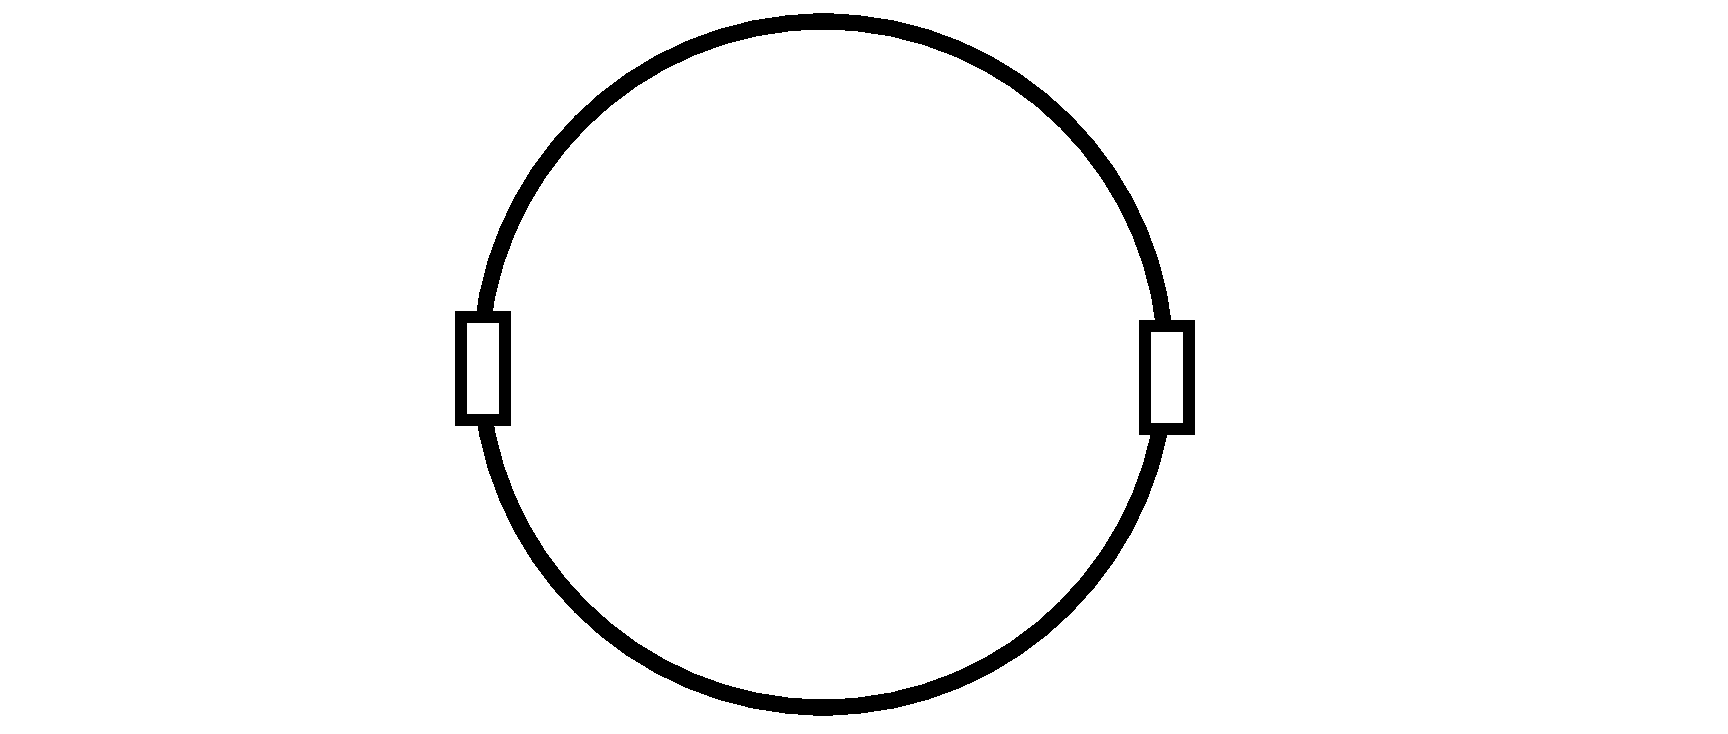
\includegraphics[width=\unitlength,page=1]{res/paradoxeSpanungsmessung2.pdf}}%
	\put(0.7045381,0.1983655){\color[rgb]{0,0,0}\makebox(0,0)[lt]{\lineheight{1.25}\smash{\begin{tabular}[t]{l}$R_2$\end{tabular}}}}%
	\put(0.21171265,0.20167302){\color[rgb]{0,0,0}\makebox(0,0)[lt]{\lineheight{1.25}\smash{\begin{tabular}[t]{l}$R_1$\end{tabular}}}}%
	\put(0.39689155,0.27113165){\color[rgb]{0,0,0}\makebox(0,0)[lt]{\lineheight{1.25}\smash{\begin{tabular}[t]{l}$-\frac{\partial \vec{B}}{\partial t}$\end{tabular}}}}%
	\put(0,0){\includegraphics[width=\unitlength,page=2]{res/paradoxeSpanungsmessung2.pdf}}%
	\put(0.06575846,0.1971287){\color[rgb]{0,0,0}\makebox(0,0)[lt]{\lineheight{1.25}\smash{\begin{tabular}[t]{l}$U_1$\end{tabular}}}}%
	\put(0.85150847,0.20341783){\color[rgb]{0,0,0}\makebox(0,0)[lt]{\lineheight{1.25}\smash{\begin{tabular}[t]{l}$U_2$\end{tabular}}}}%
	\put(0.31981416,0.15056218){\color[rgb]{0,0,0}\makebox(0,0)[lt]{\lineheight{1.25}\smash{\begin{tabular}[t]{l}$\mathcal{E}=\oint\limits_{C(A)} \vec{E}\cdot \dd \vec{s} = -\iint\limits_A \dot{\vec{B}}\cdot \dd \vec{A}$\end{tabular}}}}%
	\put(0.32846175,0.32194138){\color[rgb]{0,0,0}\makebox(0,0)[lt]{\lineheight{1.25}\smash{\begin{tabular}[t]{l}$\mathcal{E}/4$\end{tabular}}}}%
	\put(0.35204605,0.07666474){\color[rgb]{0,0,0}\makebox(0,0)[lt]{\lineheight{1.25}\smash{\begin{tabular}[t]{l}$\mathcal{E}/4$\end{tabular}}}}%
	\put(0.57137998,0.08374004){\color[rgb]{0,0,0}\makebox(0,0)[lt]{\lineheight{1.25}\smash{\begin{tabular}[t]{l}$\mathcal{E}/4$\end{tabular}}}}%
	\put(0.56666313,0.33137513){\color[rgb]{0,0,0}\makebox(0,0)[lt]{\lineheight{1.25}\smash{\begin{tabular}[t]{l}$\mathcal{E}/4$\end{tabular}}}}%
	\put(0.19481742,0.31329384){\color[rgb]{0,0,0}\makebox(0,0)[lt]{\lineheight{1.25}\smash{\begin{tabular}[t]{l}$\mathcal{E}/4$\end{tabular}}}}%
	\put(0.19560356,0.10889662){\color[rgb]{0,0,0}\makebox(0,0)[lt]{\lineheight{1.25}\smash{\begin{tabular}[t]{l}$\mathcal{E}/4$\end{tabular}}}}%
	\put(0.69873519,0.08924303){\color[rgb]{0,0,0}\makebox(0,0)[lt]{\lineheight{1.25}\smash{\begin{tabular}[t]{l}$\mathcal{E}/4$\end{tabular}}}}%
	\put(0.69637676,0.33058898){\color[rgb]{0,0,0}\makebox(0,0)[lt]{\lineheight{1.25}\smash{\begin{tabular}[t]{l}$\mathcal{E}/4$\end{tabular}}}}%
\end{picture}%
\endgroup%
}
		        \end{center}
		        In der schwarzen Leiterschleife gibt es eine eingeprägte elektrische Feldstärke durch die Induktion, welche zu einem Stromfluss führt. Da die blau-grüne Schleife nicht geschlossen ist, hier kann trotz induzierter Spannung kein Strom fließen. Es werden folgende Annahmen getroffen:
		        \begin{itemize}
		        	\item Die Leiter der Schleife sind ideal, sodass es keinen Spannungsabfall durch Stromfluss in diesen Gebieten gibt.
		        	\item Die Fläche der schwarzen Schleife entspricht der Fläche der blau-grünen Schleife. In beiden Schleifen wird so die selbe induzierte Spannung hervorgerufen.
		        	\item Die Widerstände und Spannungsmesspunkte haben eine Größe $g$, welche wesentlich kleiner ist, als der Umfang der Gesamtschleife $l$, also $l\gg g$. Der Anteil der Urspannung, der auf diese Bereiche entfällt, kann entsprechend $\frac{g}{l}\mathcal{E}\approx 0$ vernachlässigt werden. Der Anteil der Urspannung, welcher auf die Leiterbereiche entfällt, ist dann aus Symmetriegründen jeweils $\frac{l/4}{l}\mathcal{E}=\frac{\mathcal{E}}{4}$.
		        	\item Die Spannungsmessung erfolgt ideal, der Widerstand der Voltmeter ist unendlich groß.
		        \end{itemize} 
		         Mit dem Kirchhoffschen Maschensatz ($\nearrow$\ref{masche}) folgt:
		        \begin{equation}\begin{split}
				        \mathcal{E} + I (R_1+R_2)= 0 \quad U_1+\mathcal{E} + I R_2 = 0 \quad -U_2+\mathcal{E} + I R_1 = 0 \to \boxed{\frac{U_1}{U_2} = -\frac{R_1}{R_2}}
			        \end{split}\end{equation}
		        Das selbe Ergebnis zeigt sich im übrigen, wenn man das Magnetfeld ausschaltet und die $\frac{\mathcal{E}}{4}$ durch konzentrierte Quellen hervorruft. Dann erfolgt die Spannungsmessung auch nicht mehr an \enquote{identischen} Punkten, denn zwischen den schwarzen Punkten und den Messpunkten sind Spannungsquellen. Die wesentliche Erkenntnis ist, dass die induzierte Spannung $U_\text{ind}$ \textbf{keine} Spannung im Sinne einer \textbf{Potentialdifferenz} ist, sondern eine \textbf{Urspannung}. Welche Gleichung in \ref{masche} genommen hängt von der Zählpfeilrichtung ab. Ist die Zählpfeilrichtung in Feldrichtung, ist mit der linken Gleichung mit $\mathcal{E}\leftrightarrow U_Q$ zu rechnen, sonst mit der rechten und $\mathcal{E}\leftrightarrow V$. In \ref{Urspannung} wird detaillierter auf die durch Induktion eingeprägte Feldstärke $E_\mathrm{E}$ und die durch Ladungstrennung hervorgerufene Feldstärke $E$ eingegangen.
  \subsubsection{Anordnungen mit Relativbewegung}
  Es gebe zwei Regionen, links gebe es ein von 0 verschiedenes, zeitlich konstantes Magnetfeld, rechts sei das Magnetfeld 0. Die Schleife wird mit der Geschwindigkeit $v$ aus dem Magnetfeld herausgezogen. Dabei wird die Spannung gemessen. Solange ein Teil der Schleife noch im Feld ist, wird eine Spannung angezeigt.
	  \begin{center}
		  \resizebox{.3\textwidth}{!}{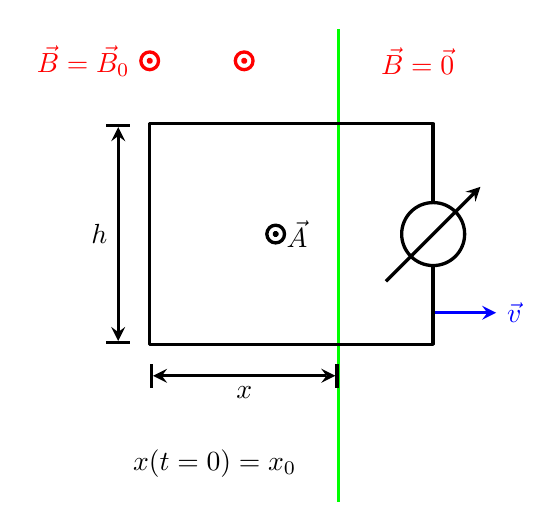
\begin{tikzpicture}[line width = 1.2pt, line join=round,x=1cm,y=1cm,>=stealth, scale = 0.4]
	% Grenzfläche
	\draw [color = green] (0,-5) -- (0,10);
	% Geschwindigkeit
	\draw [color = blue,->] (3,1) -- ++(2,0) node [anchor = west] {$ \vec{v} $};
	% Leiterschleife
	\draw (-6,0) rectangle (3,7);
	\filldraw [fill = white, draw = black] (3,3.5) circle (1);
	\draw [->] (1.5,2) -- ++(3,3);
	% Normalenvektor der Fläche
	\coordinate (a) at (-2,3.5);
	\filldraw (a) circle (1.5pt);
	\draw (a) circle (8pt);
	\draw (a) node [anchor = west] {$ \vec{A} $};
	% Höhe der Schleife
	\draw [|<->|] (-7,0) -- ++(0,7) node [anchor = east, midway] {$ h $};
	% Durchflossene Schleife
	\draw [|<->|] (0,-1) -- ++(-6,0) node [anchor = north, midway] {$ x $};
	\draw (-1,-3) node [anchor = north east] {$ x(t = 0) = x_0 $};
	% Magnetisches Feld
	\coordinate (ma) at (-6,9);
	\coordinate (mb) at (-3,9);
	\coordinate (mc) at (1,9);
	\draw [color = red] (ma) circle (1.5pt);
	\draw [color = red] (ma) circle (8pt);
	\draw [color = red] (ma) node [anchor = east] {$ \vec{B}  = \vec{B} _0\  $};
	\draw [color = red] (mb) circle (1.5pt);
	\draw [color = red] (mb) circle (8pt);
	\draw [color = red] (mc) node [anchor = west] {$ \vec{B}  = \vec{0} $};
\end{tikzpicture}}
	  \end{center}
		   Offenbar gilt  hier $\frac{\partial \vec{B} }{\partial t} = \vec{0}$, sodass:
		        \begin{equation}\begin{split}\label{scheinparadox}
				        \to \oint\limits_{C(A)} \vec{E}\cdot\dd\vec{s} = -\iint\limits_{A} \frac{\partial \vec{B} }{\partial t} \cdot \dd \vec{A} = 0
			        \end{split}\end{equation}
		   Das Experiment zeigt, dass \textbf{eine Spannung induziert} wird. Erklären kann man das beispielsweise über die \textbf{Lorentzkraft} auf Ladungsträger im bewegtem Leiter ($\nearrow$\ref{lorentz}). Das ist hier vollkommen zulässig, aber wenn die Leiterschleife weggelassen wird, muss trotzdem eine Induktion im Sinne einer eingeprägten Feldstärke stattfinden. Insbesondere für elektromagnetische Wellen (also Kommunikationstechnik) ist es essentiell, dass das Induktionsgesetz auch ohne vorhandene Ladungsträger funktioniert. Das Problem lässt sich auf zwei Arten lösen:
		          \begin{enumerate}
			        \item \textbf{Mathematisch} mit der vollständigen \textbf{Leibniz-Regel für Integrale}
			        \item \textbf{Physikalisch} mit der \textbf{Speziellen Relativitätstheorie}
		        \end{enumerate}
	  \textbf{1. Leibniz Integralregel (mathematisch):}\\
			  Der eindimensionale Fall dieser Regel lautet:
			        \begin{equation}\begin{split}
					        \frac{\dd}{\dd t} \left( \int\displaylimits_{a(t)}^{b(t)} f(t,x)\dd x \right) = f(t,b(t)) \frac{\dd }{\dd t}b(t)  - f(t,a(t)) \frac{\dd }{\dd t}a(t) +  \int\displaylimits_{a(t)}^{b(t)} \frac{\partial}{\partial t}f(t,x)\dd x
				        \end{split}\end{equation}
			  Das kann man auch in 3D übertragen, dann gilt (Beweis: Flanders - \enquote{Differentiation under the Integral Sign}):
			        \begin{equation}\begin{split}
					        \frac{\dd}{\dd t}  \iint\limits_{A(t)} \vec{f} (\vec{r} , t) \cdot \dd\vec{A} = \iint\limits_{A(t)} \left( \frac{\partial}{\partial t}\vec{f}(\vec{r} , t) + \left[ \div \; \vec{f}(\vec{r} , t) \right] \vec{v} \right) \cdot \dd\vec{A} - \oint\displaylimits_{C(A(t))}
					        \vec{v} \times  \vec{f}(\vec{r} , t) \cdot \dd\vec{s}   \end{split}\end{equation}
			 Hier ist \(\div \vec{B} =0\), also:
			        \begin{equation}\begin{split}
					        \frac{\dd}{\dd t}  \iint\limits_{A(t)} \vec{B}  (\vec{r} , t) \cdot \dd\vec{A} = \iint\limits_{A(t)} \frac{\partial}{\partial t}\vec{B} (\vec{r} , t) \cdot \dd\vec{A} - \oint\displaylimits_{C(A(t))}
					        \vec{v} \times \vec{B} (\vec{r} , t) \cdot \dd\vec{s}   \end{split}\end{equation}
			  Damit folgt dann (oft werden die Terme im Integral \enquote{Ruhe- und Bewegungsinduktion} genannt):
			        \begin{equation}\begin{split}
					        \boxed{\mathcal{E}=U_\text{ind} = \oint\displaylimits_{C(A(t))} \left( \vec{E} + \vec{v} \times \vec{B} \right) \cdot\dd\vec{s} = - \frac{\dd}{\dd t}  \iint\limits_{A(t)} \vec{B}  \cdot \dd\vec{A}  = -\dot{\Phi}}
				        \end{split}\end{equation}
	  \textbf{2. Spezielle Relativitätstheorie (physikalisch):}\\
			  Die spezielle Relativitätstheorie wird in \ref{SRT} aufgegriffen. Genutzt werden dort unter anderem die folgenden beiden Faktoren:
			        \begin{equation}\begin{split}
					        \beta = \frac{v}{c},\quad \beta \in [0, 1]\quad\quad \text{ und }\quad\quad \gamma = \sqrt{\frac{1}{1-\beta^2}},\quad \gamma \in [1,\infty)
				        \end{split}\end{equation}
			        \begin{center}
			        \begin{tabular}{c||c|c|c|c|c|c |c|c|c|c}
				        $\beta$  & 0 & 0.1   & 0.2   & 0.3   & 0.4   & 0.5   & 0.6  & 0.8   & 1.0      \\
				        \hline
				        $\gamma$ & 1 & 1.005 & 1.021 & 1.048 & 1.091 & 1.155 & 1.25 & 1.667 & $\infty$
			        \end{tabular}
			        \end{center}
			  Eine gute Näherung für nicht-relativistische Geschwindigkeiten ist {$\gamma = 1$}, mit der hier weiter gearbeitet wird. Es sei $S'$ ein Inertialsystem, das sich mit $\vec{v}=\text{const.}$ relativ zum Laborsystem $S$ bewegt (Ruhesystem der Schleife). Mit $\vec{v} = v \vu{v}$ können die Felder in $S$ in longitudinale und transversale Anteile zerlegt werden:
			        \begin{align}
				        \vec{E} & = \vec{E}_\parallel + \vec{E}_\perp = (\vu{v} \cdot \vec{E}) \vu{v} + \vu{v} \times (\vu{v} \times \vec{E})     \\
				        \vec{B} & = \vec{B} _\parallel + \vec{B} _\perp = (\vu{v} \cdot \vec{B} ) \vu{v} + \vu{v} \times (\vu{v} \times \vec{B} )
			        \end{align}
			  Im System $S'$ ergeben sich diese Felder dann nach Lorentztransformation zu:
			        \begin{align}
				        \vec{E}' & = \vec{E}_\parallel + \gamma ( \vec{E}_\perp + \vec{v} \times \vec{B} )                                                             & \vec{B} ' & = \vec{B} _\parallel + \gamma ( \vec{B} _\perp - \frac{1}{c^2}\vec{v} \times \vec{E})\label{allglorentz} \\
				                 & = (\vu{v} \cdot \vec{E}) \vu{v} + \gamma \left[\vu{v} \times (\vu{v} \times \vec{E}) + \vec{v} \times \vec{B}  \right]              &
				                 & = (\vu{v} \cdot \vec{B} ) \vu{v} + \gamma \left[\vu{v} \times (\vu{v} \times \vec{B} ) - \frac{\vec{v}}{c^2} \times \vec{E} \right] \nonumber
			        \end{align}
			  Für $v \ll c$ folgt für die Felder im Ruhesystem der Schleife ($S'$):
			        \begin{align}
				        \vec{E}_\parallel' & = \vec{E}_\parallel                      & \vec{B} _\parallel' & = \vec{B} _\parallel \\
				        \vec{E}_\perp'     & = \vec{E}_\perp + \vec{v} \times \vec{B} & \vec{B} _\perp'     & = \vec{B} _\perp
			        \end{align}
			   Es gilt wegen $\gamma=1$, dass $t=t'$, $\vec{B}(\vec{r},t)=\vec{B}'(\vec{r}',t)$ und $\vec{E}(\vec{r},t)+\vec{v}\times\vec{B}(\vec{r},t)=\vec{E}'(\vec{r}',t)$, aber $\vec{0}=\frac{\partial\vec{B}(\vec{r},t)}{\partial t}\neq\frac{\partial\vec{B}'(\vec{r}',t)}{\partial t} $. Es folgt unter Ausnutzung von $A'\neq f(t)$ (was ermöglicht die Differentiation vor das Integral zu ziehen):
			        \begin{equation}\begin{split}
			        \oint\limits_{C( A(t))}\left(\vec{E}+\vec{v}\times\vec{B}\right)\mathrm{d} \vec{s}=	\oint\limits_{C (A')}\vec{E}'\mathrm{d} \vec{s}'=-\iint\limits_{A'} \frac{\partial \vec{B}'}{\partial t}\mathrm{d} \vec{A}'&=-\frac{\mathrm{d}}{\mathrm{d} t}\iint\limits_{A'} \vec{B}'\mathrm{d} \vec{A}'=-\frac{\mathrm{d}}{\mathrm{d} t}\iint\limits_{A(t)} \vec{B}\mathrm{d} \vec{A} \\
			        		&\neq -\iint\limits_{A(t)} \frac{\partial \vec{B}}{\partial t}\mathrm{d} \vec{A}\\
					        \Aboxed{U_\text{ind} = \oint\displaylimits_{C(A(t))} \left( \vec{E} + \vec{v} \times \vec{B} \right) \cdot\dd\vec{s} &= - \frac{\dd}{\dd t}  \iint\limits_{A(t)} \vec{B}  \cdot \dd\vec{A}  = -\dot{\Phi}}
				        \end{split}\end{equation}
			 Mathematik (pure Logik) und Physik (aus Beobachtung abgeleitete Theorie) liefern \textbf{identische Resultate}! Die sich ergebende Gleichung ist für den Fall einer Leiterschleife auch wie oben erwähnt über die Lorentzkraft erklärbar. Wegen \ref{scheinparadox} folgt wenn $\frac{\partial \vec{B}}{\partial t}=0$ ist, dass $\oint \vec{E}\dd \vec{s}=0$ ist. Die induzierte Spannung wird dann nur noch durch den Term der Lorentzkraft hervorgerufen, was intuitiv erscheint, weil durch diese Kraft Ladungsträger so verschoben werden, dass sich eine Spannung aufbaut.
		  